\pdfoutput=1

\documentclass{l4proj}
\usepackage{float}
\usepackage{hyperref}
\usepackage{lscape}
\usepackage{rotating}
\usepackage{multirow}
\usepackage{booktabs,caption}
\usepackage[table,xcdraw]{}
\usepackage{wrapfig}
\usepackage[compact]{titlesec} 
\usepackage[table]{xcolor}
%\usepackage{alltt}

%\usepackage{fancyvrb}
%\usepackage{bera}

%
% put any packages here
%

\begin{document}
\title{Are matrix-based or node-link graphs more readable when representing causal relationships for social and health data?}
\author{Kristina Lazarova}
\date{March, 2017}
\maketitle

\begin{abstract}

People who work in the social and health policy make decisions based on causality. Causality is usually visualised by node-link graphs, but matrix-based representations have the potential to outperform them because of their concise and clear visual representation. However, matrix-based graphs have not been extensively studied in causal relationship visualisation. Therefore, an experimental software was created to test human performance on reading causal relationships in node-link and matrix-based graphs. To make a thorough investigation of the factors influencing reading time different sizes, layouts and type of questions were created. Response time and correctness of the answer were measured. The results showed that matrix-based graphs outperforms node-link representations in direct questions. When path questions are concerned, however, node-link graphs were found to be more readable than matrix-based graphs. (DISCUSSION) 
 
\end{abstract}

\educationalconsent
%
%NOTE: if you include the educationalconsent (above) and your project is graded an A then
%      it may be entered in the CS Hall of Fame
%
\tableofcontents
%==============================================================================
\chapter{Literature Review}
\pagenumbering{arabic}

\section{Data Visualisation}

Data visualisation has been described as a technique that makes use of computer-supported, interactive illustrations to deepen human's understanding of a dataset \cite{card1999readings}. Information visualisation (InfoVis) is necessary when dealing with increasingly large and complex data. InfoVis systems are most helpful when a set of data is being explored \cite{fekete2008value}. Usually this occurs not when someone is looking for a specific answer to a question, but when a deeper understanding of that data set is sought. It was suggested that the value of information visualisation is not in understanding a specific question, it is about developing and deepening one's insights of a set of data \cite{fekete2008value}. Data visualisation is able to facilitate this process because there are a number of cognitive benefits associated with it. A large visual cue that illustrates data becomes a single point of reference for human cognitive processes. Visuals become external cognition helpers in facilitating human memory by providing a bigger working set for analysing data. 

Density of the InfoVis and task difficulty are known to influence human performance \cite{netzel2014comparative}. For instance, following a single path on a graph with one trajectory would require less cognitive effort than performing the same task on a highly dense and complex network. However, the exploration of a representation can convey a better insight into the meaning of the data \citep{al2014information}. Al and colleagues \citep{al2014information} argues that InfoVIs has three main roles: communication field, knowledge management mean, and decision support instrument. Furthermore, visual architecture and design applied at company and department levels have been reported to be successful due to the low cognitive burden for visualization reading \cite{king2016cognitive}.

Data visualisation has been been used in a number of fields. For example, it is suggested to be successfully used in Bank of America Chicago Marathon, which is one of the biggest marathons in the world \cite{hanken2016developing}. Large amounts of live data are gathered to establish some of the main principles for event management information visualization. The main benefits from these practices are keeping track of the progress of the participants, communicating information between the agencies organizing the marathon efficiently, and improving medical preparedness. 

Moreover, astronomical researchers have been suggested to benefit from data visualization techniques \cite{goodman2012principles}. One such technique is linked views in which a user is able to select, highlight and include or exclude points from display and analysis from various data visualisation dimensions. For example, an important visualisation for astrologists can be interactive exploration of relationships between data points in statistical graphs and locations in live 3D space. Another instance of beneficial data visualisation is "Geographic Information System" tools which are used in demographics and geography. For example, Engage3D provides the functionality of exploring layers of maps in a linked-view systems. 

Inventions in this field have been continuously made in order improve the visualisations and benefit the target public. For example, a heatmap represents a graphical illustration that evaluates conical distribution values around data points based on a respective data value that has associated respective data point \cite{cardno2014data}. Various implementations of a heatmap were developed and discussed since the original heatmap was created, in order to enable easy future work with heatmaps suited for a particularly needed area.

There have been data visualisation issue related to Big Data \cite{gorodov2013analytical}. First, visual noise is the phenomenon of having so many data points on the screen that the user cannot see them as separate points which leads to visibility loss. Second, large images are dependent on the device's resolution abilities. However, even if many devices are added together for partial data visualisation to represent a more detailed illustration or a larger amount of data, human perception will eventually reach its limit. Therefore, after a certain point people will not be able understand the representations or their analysis. A third problem is information loss which is caused by data filtration and aggregation. These techniques are likely to hide information and mislead people analysing the data. Another problem is High Performance Requirements especially in dynamic visualization. In addition, the visualisation might be accompanied by high rate of image change and lead to people being unable to react to the number of data changes. 

A Big Data visualization method is suggested to be TreeMap \cite{gorodov2013analytical} which is a hierarchical way of representing data by rectangles. Some advantages of this method are that the hierarchical matching clearly shows data relations and extreme outliers are visible. The disadvantages related to this method are that the data must be hierarchical which makes it unsuitable for examining time patterns, for example. 

A well-known issue if InfoVis is that sometimes it is challenging for people to understand it. A study aimed to examine familiarity of museum visitors with different visualisation techniques \cite{borner2015investigating}. They included charts, maps, graphs, and networks to reveal how familiar people are with them. It was found that even though most participants were interested in science and art they had difficulties naming and reading the visualisations. It was concluded that people are interested in visualisation techniques, but have significant difficulties in naming and understanding them. 

In order to solve this issue, research has also investigated the way InfoVis novices approach reading data and the methoths that can facilitate their learning. A study used sales data to find the barriers for novices when reading iterative visualisation construction and the way they think about visualisation specifications \cite{grammel2010information}. They found that the biggest barriers were interpreting questions into data factors, visual mappings, and understanding the visual representations. It was found that there is a need for instruments that suggest possible visualizations, facilitate help with learning, and are integrated with tool support for the whole analytic process. Furthermore, recent research acknowledged that individual differences between people will have influence on the way they interpret graphical representations \cite{Steichen:2013:UIV:2449396.2449439}. They suggested that visualization performance can be improved by personalising visuals according to one's needs, abilities and preferences.

Very little is known about the way users understand and read data visualisations and how they interact with different layouts \cite{etemadpour2015perception}. It is interesting to explore if there are layouts which provoke better task performance and better response time. Etemadpour and colleagues \cite{etemadpour2015perception} conducted a research to find out more about performance in similarity based layouts that are generated by multidimensional projections. The results suggested that projection performance is task-dependent and depends on the nature of the data. Therefore, they concluded that the same data layout can have different performance on different tasks and that performance will also be influenced by the characteristics of the data.

\section{Causal Relationships}

Causal relationships are of great interest for scientist who examine influence of different factors on each other. Particularly, research regarding health, social and behavioural sciences aim to investigate questions about causal rather than associative relationships. With the help of statistical analysis associations among different factors can be inferred. Associations are relationships that can be observed in joint distributions of factors such as regressions and correlations. Causal analysis, in addition, is the practice that aims to infer probabilities under factors that are changing \cite{pearl2010introduction}. These could be, for example, changes influenced by factors such as drinking, childhood issues or applied treatments.  

A study looking to identify factors influencing blog design used the Decision Making Trial and Evaluation Laboratory method (DALMATEL) which is used to illustrate the relationships between factors and allows causal relationships to be shown \cite{hsu2012evaluation}. Some of the causal relationships they found were that color arrangement directly impacts simplicity of layout, colour arrangement directly impacts font arrangement, and color arrangement impacts itself. 

ReView is a tool for finding causal relationships in anomalies in network traffic. It has been suggested to facilitate better understanding of network representations \cite{Zhang:2015:VTC:2713579.2713583}. One of its features is minimizing the detailed information while showing the causal relationship. ReView can also quickly navigate the user through networks with a large number of requests and levels of abstractions.

Causal relationships are thought to be perceived easier if they are accompanied by animation. Ware and colleagues \cite{ware1999visualizing} followed Michotte's perception of causality principle which illustrates a causal event with a billiard ball hitting another ball and causing its motion. They introduced a visual causal vector method that shows a causal relationship between representations using animation. They found that the perception of causality depends on the simultaneous occurrence the visual causal vector and the change in the graphical representations. 

\section{Node-Link Graphs}

Node-link graphs consist of nodes which are connected by edges. Large amount of work has been dedicated to visualizing those structures in the most readable way. However, the larger the network that is being illustrated, the higher the possibility that the graph becomes dense and unreadable. This is especially true when the direction of the edges is important \cite{dwyer2013edge}. When representing causal relationships with node-link graphs if node n is causing node m, then the edge between those two nodes will point towards node m. In order to avoid the complexity of the large network some researchers have tried to add interaction with the graph \cite{gansner2005topological}, while others' intention was to create visuals that do not change the structure of the network and does not require interaction \cite{dwyer2013edge}. An innovative interaction technique was designed by Abello et al \cite{abello2006ask} where a user is able to navigate through a hierarchically clustered base of the graph. In the noninteractive technique researchers decreased the complexity of large directed graphs by replacing single edges with edges which connect to groups of nodes \cite{dwyer2013edge}.  

Data driven journalism is also concerned with difficulties in showing directed relationships in large datasets \cite{niederer2015survey}. Nodes have also been used to represent "visual programming language" or workflow and processing functions \cite{thattai2016systems}. The system translates the user input into "a sequence of data language", which will then be transformed into "service commands" that will be executed. The dependencies between the nodes and data flows are illustrated as interconnections between the vertices on the graphical user interface. 

A collider "C" is well represented by an "inverted fork", $A->C<-B$, in which the arrow shows a direct link from the tail factors to the head factor \cite{greenland2003quantifying}. Stratifying on the collider is likely to induce bias and influence the the association between A and B. In addition, a similar pattern found in directed acyclic graphs, called a confounder, can be illustrated by a "causal fork" - $A<-C-> B$. Greenland \cite{greenland2003quantifying} suggested that any change in the A-B link upon C-stratification will induce bias. Statistical adjustment for collider bias is suggested to lead to as much bias as not making adjustments for a confounder \cite{janszky2010janus}. 

Directed acyclic graphs (DAGs) are increasingly used in representing causal relationships in modern epidemiology \cite{suttorp2015graphical}. The factors in DAGs are connected by arrows which can never create a closed loop \cite{greenland1999causal}. A path is defined by a sequence of arrows between the factors of interest. The DAG method is valuable as it is found to show underlying relations explicitly and easily identifies sources of confounding. A confounder is known to be a variable that is related with the exposure and the outcome but does not exists in the causal path between them. For example, chronic kidney disease and mortality are often caused by age. Confounding occurs when reading the causal relationships between chronic kidney disease and the outcome mortality. 

Directed node-link graphs are often used to represent causal data. Dense node-link diagrams make rading graphs harder and colliders and confounders are known for inducing reading biases. However node-link graphs are among the visualisations that do not require extensive learning and are easy and intuitive to read, as they fit the structure of the mental represetation they visualise\cite{netzel2014comparative}.

\section{Matrix-based Graphs}

An Adjacency matrix is frequently used to represent a network \cite{longabaugh2012combing}. Matrices can be used to represent both directed and undirected graphs. If a network consists of n nodes, the matrix will consists n x n grid of cells. A new technique called Compressed Adjacency Matrices was introduced in 2012 for visualising gene regulatory networks \cite{dinkla2012compressed}. As those directed networks have specific structural traits, standard representations such as adjacency matrices, and node-link diagrams are unable to depict all traits. Compressed Adjacency Matrices cut and rearrange adjacency matrix so that no space is wasted in case of sparse network. There are specific structures which represent sub networks. This is how scientists came up with a new data structure in order to fit the characteristics of the data they analyse.

Furthermore, PathwayMatrix is another visualisation tool that represents specific relations between proteins in a pathway \cite{dang2015pathwaymatrix}. The implementation of the tool consists of adjacent matrices that interact with each other. Additional features were added to facilitate the data analysis. This visualisation software received positive feedback in the specific area of representing relations in proteins pathways. Consequently, there is no one best representation technique. Depending on the dataset specifications, the complexity and size of the data there might be many or only few sufficient ways to visualise it.       

A performance comparison between square and triangular matrices has been conducted to measure performance speed and accuracy \cite{liu2015effects}. It was found that performance is influenced by the matrix juxtaposition type which lead to the creation of a new matrix visualisation called TileMatrix. It represents a large amount of matrices and is effective at analysing networks that are multi-faceted and time-varying. With TileMatrix it is easy to see differences in matrices across time and facets. However, triangular matrices can work only in non-directed networks. 

On the other hand, some of the disadvantages of matrix-based graphs are that the area increases quadratically and as large networks are sparse there will be mainly empty space on the matrix. Improvements such as compressed adjacency matrix try to account for some of these disadvantages and in general matrix-based representations are considered to be an unambiguous and concise way of representing data. The main advantages of a matrix-based graph are that it has no overlapping and can be ordered.

\chapter{Introduction}

Alper and colleagues \cite{alper2013weighted} compared augmented adjacency matrix with node-link visualization in brain connectivity by conducting a controlled experiment. Brain connectivity visualisations are in the form of weighted graphs which are node-link graphs in which each edge is given a numerical weight. They found that matrix-based graphs outperform node-linked graphs. It was concluded that for weight graphs, node-link representations are less readable and more error-prone when compared to matrices. On the other side, node-link graphs are adjustable to a specific spacial representation which might also be insightful when reading the graph. Overall, matrix-based graphs had higher accuracy.  

Furthermore, it was suggested that adjacency matrices are superior to node-link graphs in representing dense graphs because they are more compact and easier to look at \cite{sheny2007path}. However, they also found that node-link graphs are better for path finding as a path can easily be followed if the arrows are not too tangled. Consequently, as mentioned earlier a unique best InfoVis does not exists. Depending on the data size, data characteristics and question of interest different representations can fit the best performing model. 


Adjacency matrices and node-link diagrams have been compared in another study \cite{keller2006matrices} to examine which is more suitable graphical representation for the general public. This research was provoked by the fact that matrices are mainly use in engineering area, while node-link graphs are generally a more popular way of visualisation. The research questions being examined were related to the attributes of the connectivity model influencing readability and which representation is more suitable for particular tasks. In addition, they filled the gap in previous research that did not take into consideration participants' familiarity with the data sets. It was found that error rates and response time are highly influenced by size and density. They confirmed Ghoniem's \cite{ghoniem2004comparison} findings that matrix-based graphs outperform node-link graphs for dense and large graphs, and node-link graphs are more readable for small and sparse graphs. The only exception found is finding the path between two nodes in a graph. Furthermore, experience with the data set showed to has effect on performance. 

Ghoniem and colleagues \cite{ghoniem2004comparison} made a performance comparison between node-link and matrix-based graphs. They predicted that counting nodes should be equally difficult on types of representations, but counting links and finding the most connected node should be easier in matrix-based representations. Node-link graphs were hypothesised to be better when building a path between two nodes. The reason for this is that matrix based graphs have the nodes represented twice which introduces extra complexity. They also hypothesised that node-link graphs will be easier to work with when dealing with graphs with a small amount of nodes. In their experiment they had three sizes of graphs - 20, 50, and 100 nodes. They tested 36 participants and measured their performance on various tasks such as finding paths, neighbours, nodes and links between nodes. They found that performance in node-link graphs decreases as the size of the graph increases. This pattern was confirmed for all of the tasks except for finding path, where node-link graphs regardless of the size and density showed better results.

\section{Aims and Objectives}

The present research question aims to investigate readability of node-link and matrix-based graphs when representing causal relationships. As discussed above the two types of representations have already been compared for non directed networks, but there is a gap in the literature that discusses their performance in causal relationships. Therefore, it is important to investigate whether their readability in directed graphs will be influenced by the same factors as in non-directed visualisations. What is more, deeper knowledge of the difference in their performance can benefit those working in the social and health policy sectors. They need an accurate and efficient way of representing data in order to make a well-informed and quick decisions. The importance of their tasks is caused by the fact that they can directly influence health policies. In addition, the health and safety sector invest large amounts of money based on their interpretation of the causal relationships graphs they posses.

Therefore, knowing which type of causal visualisation is more efficient and accurate will help the health sector make correct and quick decisions. As discussed earlier there can be a best performing visualisation each type of task. To broaden our understanding of the factors that influence readability different factors can be manipulated during the experiment: type of task, question asked, graph layout and size. In order to find the answer to that research question an experimental software needs to be implemented. It needs to allow the researcher to add the questions of interest with corresponding graphs and the participants to answer them. To measure performance, the software must measure time to answer the question, and whether the answer is correct. The results of the experiment will show whether node-link or matrix-based graph is better at representing causal relationships. Also it will become clear if any significant performance difference is modulated by factor such as layout and size of the graphs. 

\chapter{Implementation details}

\section{Requirements}

The first step of the implementation was understanding the system that needs to be created. In order to test the proposed research question an web application had to be created where participants can give answers to the data visualisation questions of interest. They were required to see a graph and a question related to the graph. The participants' response time had to be recorded as well as whether their answer is correct. At the same time, the experimenter need to be able to check the participants' answers to the questions. After considering all requirements, a user story for each feature was created. Some of the most important user stories are:

\begin{itemize}
   \item As a researcher, I want to be able to see participant's answers to questions, so that I can analyse the data.
   \item As a participant, I want to be able to see a graph and a questions at a time, so that I can complete the experiment.
   \item As a researcher, I want to keep participant's scores anonymous, so that the experiment comply with ethics requirements.
   \item As a participant, I want to be unable to go the next question before completing the present question, so that I am certain that I haven't missed a question.
   \item As a researcher, I want to be able to see participants' demographic information, so that I can make generalisations about my experiment.
\end{itemize}

\section{Prototype}
After the requirements gathering analysis, development of wire-frames followed. Balsamiq Mockups 3 was the software used for the creation of wire-frames. An example of the research question page can be found in figure \ref{researchQuestion}.

\begin{figure}[H]
\centering
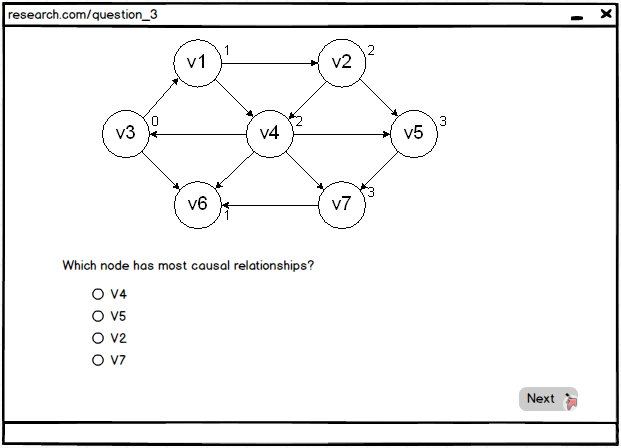
\includegraphics[width=9cm,height=7cm]{researchQuestion.PNG}
\caption{Research Question Wire-frame}
\label{researchQuestion}
\end{figure}
 
After discussing the wire-frames it appeared that some important features are missing. One of those features was a participants training session. The aim of the experiment is to test which graph is more readable for people who do not have regular exposure to such data visualisation. Therefore, it is important to make the participants aware of how to read each graph before the actual experiment. This is how the requirements specification became an iterative process during which a better understanding of the product evolved.

\section{Software tools and technologies}

Choosing the appropriate tools and technologies for this project was an exciting task. However, taking the right decisions was a long process. After a research period followed by a trial-error week it was decided that the backend of the application will built with Node.js and JavaScript combined with the web application framework Express. Node.js was chosen on the grounds of being event-driven, non-blocking I/O model which contributes to a very efficient and lightweight software. A Node.js JavaScript engine is used in the Google Chrome browser and has a very good performance \cite{tilkov2010node}. JavaScript servers have incredible performance due to their asynchronous I/O. Node.js appears to be single-threaded from a developer's point of view, as there is no thread management involved in the development process. However, behind the scenes Node.js handles threading, file system events, implements the event loop, feature thread pooling etc. Coming from a Java background, the Maven equivalent in Node.js is NPM. By using NPM commands the developer is able to install variety of different modules to help the implementation process. NPM executes the function of a package manager. Express is the standard server framework for Node.js. It is usually described as a minimal and flexible Node.js web application framework. Many popular frameworks such as KeystoneJS, Kraken and Sails, are built on Express. 

AngularJS 1 was chosen for management of frontend functionality. Even though there is a newer version of the product, the lack of documentation and support online, was a sufficient reason for using the older AngularJS. It uses HTML as a template and enables the developers to extend it to express the application's components clearly. AngularJS supports features such as data binding and dependency injection which decreases the amount of code that a developer would usually write to implement them. 

The database system chosen for the project is PostgreSQL. Considering the size of the project an object-relational database was chosen. In addition, it was decided on PostgreSQL in particular because it is open source and has gained a reputation of a reliable database system. Also previous experience with PosgreSQL from developers point of view made the decision easier. The database schema looked like this:\newline \textbf{questions} (\underline{question\_id}, question, answer\_one, answer\_two, answer\_three,
		answer\_four, correct, image, type, layout, domain\_question, question\_type) \newline
\textbf{answers}(\underline{question\_id}, \underline{participant\_id}, time, correct) \newline
\textbf{participant\_info}(\underline{participant\_id}, name, email, degree) \newline
\textbf{latin\_square}(\underline{participant\_id}, sequence) \newline


\section{System Design}
Designing the system was the next stage in the process. Figure \ref{abstractDesign} shows an abstract view of the system design. There is an Actor who will either be a participant in the study or a researcher. They will interact with the frontend which will be in the form of a web application in a browser. The front end will communicate with the backend which will be implemented in Node.js. The backend will make requests to the database to retrieve and send information. 

\begin{figure}[H]
\centering
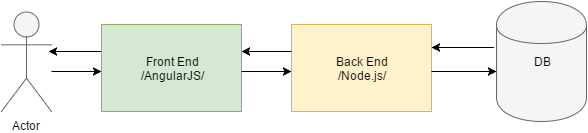
\includegraphics[width=13cm]{abstractDesign.png}
\caption{An abstract representation of the system design}
\label{abstractDesign}
\end{figure}

Figure \ref{moreSpecificDesign} displays a more detailed version of the system design. This design has been implemented to separate the different concerns in this specific system. When the Actor interacts with the application, the frontend will send information to the Controllers. There will be as many controllers as pages with front-end functionality in the web application. The Controller component decides what should the next action be according to the user input. It has control over the front-end logic and sending requests to the Service if information from the database or the server is requested. For example, the answers to all questions are kept in the front-end until a "Submit" button is clicked on. This action triggers a request to the Service. The Service component works with the back-end logic. It can send and retrieve data from the database and keep the information in the Repository. The Service also deals with the requests for the different web pages. It also ensures that the project dependencies are loaded.   

\begin{figure}[H]
\centering
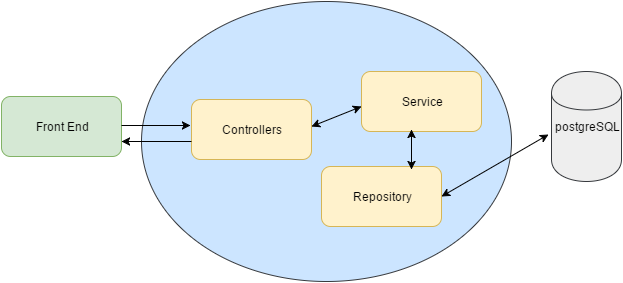
\includegraphics[width=15cm]{moreSpecificDesign.png}
\caption{A more specific representation of the system design}
\label{moreSpecificDesign}
\end{figure}


\section{Implementation}
The development process was split into frontend and backend. Without using any frameworks, the frontend HTML pages were created following the wireframes. Bootstrap was added to the HTML to improve the UI design and make it look more appealing for the participant. Furthermore, a hierarchical page set up was implemented by having all HTML pages extending one layout file. This also helped to avoid repeated code as the required libraries were imported only once and all other files inherited them. A considerable amount of time was spent on developing the graphs and converting node-link graphs into matrix-based graphs. Close to piloting the experiment an important issue was noticed. When large graphs were displayed on the web page a scrollbar had to be added in order to see the whole graph. This was going to influence the response time and therefore the front end had to be drastically changed to comply with this requirement. The bootstrap elements were slitting the page into separate well-defined components - the experimental heading, remaining time bar, an image section and a question section. After reviewing which is the necessary information on the page only the graph image and the question were left.

By this time, it was clear that Node.js will be used to create a server so the next step was to implement it. As Node.js is growing in popularity, there are a number of useful tutorials available online. Setting up a server in javaScript was exciting and surprisingly quick. Afterwards, the HTML pages were mapped to a Express handlebars or hbs files. Before implementing the functionality of the web application the database system was created and connected to the web application. Postman was used to check whether the POST requests to the database are working correctly. 

Once it was established that the skeleton of the application is working, Angular was used to do the data binding in the frontend. For each new participant, there was a participant id created, which then was related to the answers to the experimental questions, and the demographic questionnaire. Cookies were used to keep the user ID throughout the experimental session. Latin square was used to randomize the question sequence for each participant. Node.js has a Latin square module which was used to generate the different sequences. Then the matrix sequences were kept in the database and linked to a participant id ensuring that each user gets a different sequence of questions. Angular was also used for populating the website data - graph images and questions. This was done by using one page template for all questions and Angular given the required sequence of questions was displaying the appropriate information. 

\section{Challenges}

In the beginning of this project the Java framework Spring was going to be used in the implementation as it is among the most widely used frameworks in industry \cite{shiLuiLi}. This decision was supported by extensive previous experience with Java from developer's point of view and the applicability of the skills to be acquired. However, one of the reasons why Spring is used in industry is because of the large and complex systems that exist there. The Spring framework works on a very high level of abstraction where you can easily write configuration files to add dependencies from different project. Therefore, it is considered rather unfriendly for small independent projects and developers with limited Spring experience. The reasoning behind this conclusion was provoked after a couple of unsuccessful attempts to set relative paths to different CSS and JavaScript files. The issue was found to be in the web application configuration file, but also the realisation that Spring is unnecessary abstract for this project appeared.

A new research for web-application frameworks followed. Node.js backend was chosen because of its event-driven, non-blocking I/O model which creates an efficient and lightweight server-side of the application. Another challenge appeared when trying to incorporate AngularJS with Node.js. Usually in AngularJS one uses curly braces to reference data structure from the AngularJS controller. However, Node.js also uses curly brackets to reference information from the backend in the frontend. This caused a conflict between Anglular and Node.js and an Angular error. After a long research  it was found that Node.js overrides the use of curly braces and the application is not displaying Angular data as it expects it come from the backend. Unfortunately, an appropriate error message does exist and this had to be discovered during the development process. Instead of using curly brackets one can also use "ng-bind" and achieve the same result. This approached solved the issue until "ng-bind" information was needed in "ng-src" clause to display the appropriate graph image. It is not possible to use "ng-bind" inside "ng-src" so the found solution at the time was no longer solving the problem. However, as the root of the issue was known, an answer to the question was found and implemented successfully. The Angular configurations had be altered to use a different symbol not the curly brackets. Implementing this solved the problem entirely. 

Another issue was the size of the graphs. During the implementation process it was necessary for a scrollbar to appear in order to show the real size of the graphs. This was inconvenient for reading the graphs, and participants were going to need more time to read these graphs. Therefore, this was going to be a confounding variable in the experiment. In order to avoid this issue, the front-end pages had to be restructured. The bootstrap navigation bar had to be removed and the question had to be displayed on the left instead of below the graph. This also meant that this particular sequence of pages had to extend a different layout page, which does not contain the navigation bar and has a different bootstrap grid. Luckily, only one HTML page was used for the research questions and Angular was used to populate the information for the next question after the present one was answered. Therefore, very little alteration had to be made to implement these changes


\chapter{Experiment}
\section{Design}

This is a within subject design experiment with two conditions. In the first condition participants answered questions related to causal relationships in node-link graphs, while in the second one they were asked to answer questions on matrix-based representation. Each condition had four levels - size, layout, question type and question domain. The dependent variables were time taken to answer each question and correctness of the answer. The participants were also given a questionnaire which required subjective answers about their graph preferences and how they enjoy solving logical problems. 

\section{Stimuli}

To prepare the experimental stimuli, a variety of graph factors had to be addressed. First, the information complexity in all graphs had to be equal to prevent if from influencing performance time. Consequently, node-link graphs were created in yEd 3.16.1 and then converted into matrix-based representations using an XGML translation software created in Glasgow University. This is how equivalently complex node-link and matrix-based representations were created. As long as the graphs were from the same domain question and size, they represented the same information. However, each question was carefully structured to require different information to be read from the graphs to avoid learning effect. 

Furthermore, in order to create a large number of graphs, three different question themes were introduced - drinking issues, exams, and healthy/unhealthy gym behaviour. To gain a deeper understanding of which are the most influential characteristics of a graph different layouts and sizes were also implemented. The three different sizes were small, medium, and large. A small node-link graph consists of 10 vertices and 10 or 9 edges \ref{sportSmallOrganicS}. The equivalent matrix-based representation has 10 rows, 10 columns and 10 or 9 darker squares showing the causal relationships between factors \ref{studentSmallInDDS}. The medium size representations had 20 factors or 20 vertices (node-link graphs) and 20 row and columns (matrix-based graph). The large graphs had 30 variables or 30 vertices in node-link graphs and 30 row and columns in matrix representations. 


\begin{figure}[tbp]
  \centering
  \begin{minipage}[b]{0.4\textwidth}
    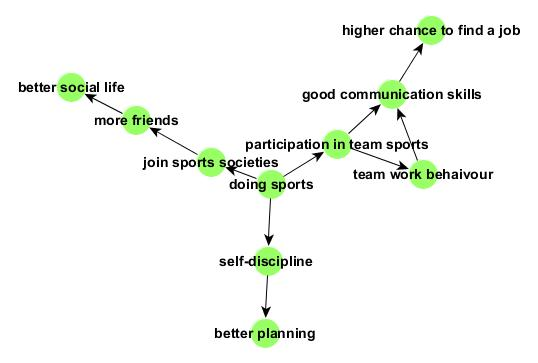
\includegraphics[width=\textwidth]{images/sportSmallOrganic.jpg}
    \caption{Small Node-link Graph}
	\label{sportSmallOrganicS}
  \end{minipage}
  \hfill
  \begin{minipage}[b]{0.4\textwidth}
    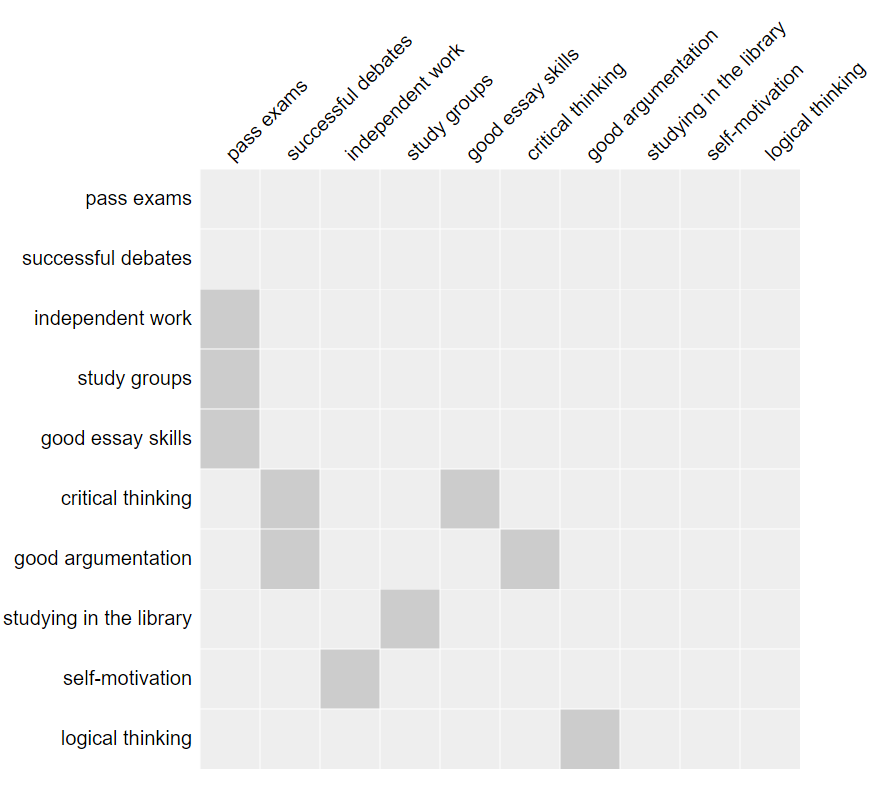
\includegraphics[width=\textwidth]{images/studentSmallInDD.PNG}
    \caption{Small Matrix-based Graph}
	\label{studentSmallInDDS}
  \end{minipage}
\end{figure}

For each type of representation different layouts were implemented. The matrix-based layouts were alphabetical, indegree descending and outdegree descending \ref{matrixLayout}. The alphabetical layout had the row and column factors in alphabetical order. The indegree descending layout finds the number of edges that are coming into each vertex and sorts them in descending order. The outdegree descending layouts calculates the amount of edges going out of each vertex and applies descending order.  The node-link layouts were hierarchical, orthogonal, and series parallel \ref{nodeLayouts}. yEd applies an algorithm for the creation of each layout. The hierarchical layout represents precedence relation in directed graphs. Series parallel graphs have one sink and source which are created recursively to generate the series parallel graph. The organic layout has well-balanced spread out distribution of nodes. Figure \ref{experimentalDesign} shows the pattern which was followed to create 36 graphs with equal amount of combinations of sizes, layouts and question domains. 

\begin{figure}[h]
\centering
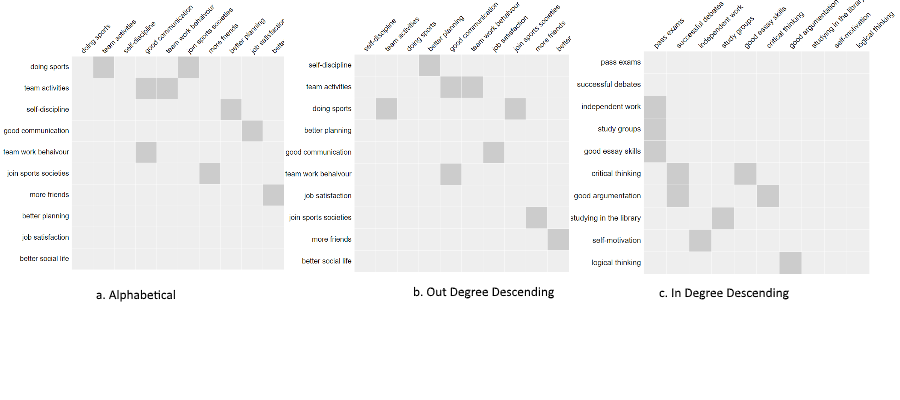
\includegraphics[width=18cm]{images/matrixLayout.png}
\caption{Matrix Layouts}
\label{matrixLayout}
\end{figure}

\begin{figure}[h]
\centering
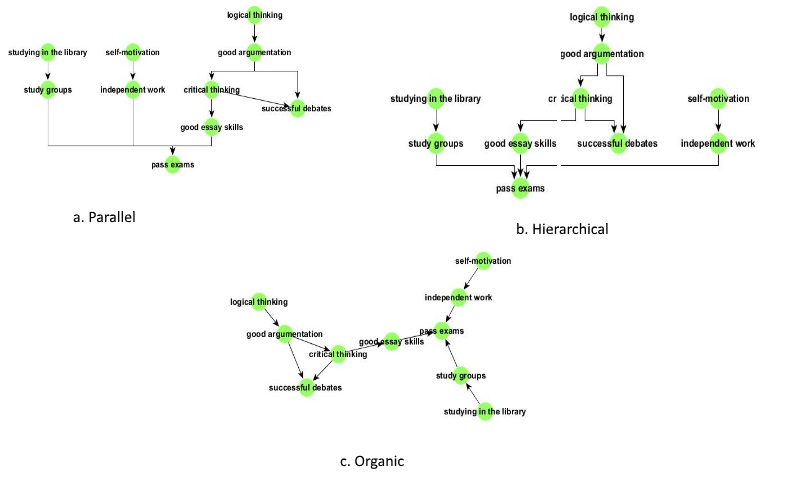
\includegraphics[width=15cm]{images/nodeLayouts.png}
\caption{Node-link Layouts}
\label{nodeLayouts}
\end{figure}

There was a direct relationship question and an indirect causal relationship question asked for each of the created graphs. The direct question was requiring the participant to answer a question of the type "Factor X is causing which of the following factors" followed by four multiple choice answers only one of which was correct. The path question was asking which of the following causal relationships is correct, followed by four multiple choice answers of the type "factor A $->$ factor B $->$ factor C". The first six questions of the experiment were training questions which did not count towards the final results. The characteristics of the graphs in these questions were chosen to be different from the graphs in the experimental questions. They were added to the beginning of the experiment which generated a total of 42 questions.

\begin{figure}[H]
\centering
\includegraphics[width=18cm]{experimentalObjects.png}
\caption{Experimental Design}
\label{experimentalDesign}
\end{figure}


The specified sequence of questions with matched layouts, question themes, and different sizes was likely to influence the results of the experiment because of the exposure effect of that particular sequence. Therefore, to ensure that all participants receive the questions in a different order, Latin square /cite{winer1962latin} randomization was used. The sequence of questions was different for each participant and the possibility of the questions sequence affecting the results was eliminated.
  
All representations were displayed in their real size on the left side of the screen and the corresponding question was on the right. A special attention was paid to the letter's font size and retaining the original size of the image on one screen. Participants were not able to go to the next question before they answered the current one. In addition, to measure answer time more accurately, there was no "Next" button. Once a participant clicked on an answer it was automatically submitted and the next question was loaded on the page. Figure \ref{exampleQuestion} in Appendix C shows an example of a trial question.

Finally, a Google Form questionnaire was used to ask participants to reflect back on their experience. Two weeks after the testing has started the participants were sent an email with the subjective questionnaire about their graph preference. 

\section{Pilot}

Conducting a pilot was an essential part of this study. It brought light into how people who have never been exposed to the graphs and the software before interact with them. It was important to learn whether the tasks are clear and the software is easy to use. Three volunteers took part in the pilot. They were asked to sit on a chair in a quiet environment and complete the experiment starting from the information sheet and finishing with the debrief form. At the end the participants were asked questions regarding the training, the clearness and enjoyment of the tasks. All participants said that the training in the beginning of the experiment is sufficient at explaining how to read the graphs. One of the participants, however, required confirmation that the correct direction of reading the graphs is from left to top. This is why, it was decided to make the first three questions trials in which the participants can ask as many questions as they need to understand how to read the graphs. The second three questions (4,5,6) were also going to be practice questions but they were not going to be explicitly informed about it. Consequently, during the first six tasks the participants were expected to fully learn how to interpret the graphs and their answers were not recorded in the results. 

An interesting problem regarding the nature of the trial questions was also considered. Initially, it was suggested that the trial instances are always the first questions of each sequence. However, as those questions would not be accounted for in the results and the Latin Square randomizes each sequence, this was going to lead to uneven number of answers for each type of graph. If this was to happen, the results of the experiment were going to be negatively influenced. In order to avoid this, 6 new questions were created using a combination of layouts, sizes and domains that has not been used for the original 36 questions. A mixture of different sizes and types was included to ensure that the participants have exposure to the main challenges of the experiment during the practice trials. These 6 questions were going to be added at the beginning of each sequence so that all participants are exposed to the same trial questions.  

All participants in the pilot said that the tasks are clear, the graphs' font size is readable, and different layouts and sizes are appropriately displaying the data. One participant mentioned that in the node-link organic layout, the label is on the arrow which makes it hard to read. The reason for this is that both labels and arrows are in black colour. Their note was taken into consideration but if changes are made to align the arrow and the label differently this would alter the organic yEd layout. Consequently, the results will provide information about a manually created layout similar to the organic yEd layout. Another solution of this issue was to change the label names to individual letters like "A" instead of actual factor labels such as "depression", and "pass exams". However, this was going to influence the complexity of the experiment and the participant's level of interest. Thus, no changes were made to the organic layout.  

One volunteer in the pilot mentioned that sometimes it is hard to find the label you are looking for and they guessed the answer to the question by logical reasoning. To avoid this problem in the experiment, a note was made to inform participants that there is no logical relationship between the causal relationships and they should not attempt to guess the correct answer. This is supposed to encourage them to look for the labels rather than guess the correct answer. 

The pilot was also extremely helpful for spotting technical issues. If it was not conducted and some of these problems were not accounted for, the recorded results would have been incorrect. First, it was found that in one question the correct answer was being evaluated to incorrect because of a typo in the csv file that was used to populate the database. In addition, the answers were not written in a consistent way, which meant that the participants might had been influenced to choose the answer that is written differently from the rest of the answers. In order to fix these problems, the database table with the questions had to be altered. 

Another technical issue found was concerned with the time recorder. It was found that the timing was starting and stopping when required, but the record of the time taken for a particular question was wrong. The issue was found to be caused by a wrong startTime variable during the timeTaken calculation. This was a scope issue, which was fixed for the real experiment. Moreover, in order to submit their answers the participants had to click a "Next" button. The timer used to stop once this button is clicked, record the time taken for the current answer, and start the timer for the next question. However, it was found that this extra click influences the recorded time and it would be more appropriate to have the time start and stop when the participants choose an answer. This led to the decision to completely remove the "Next" button and submit the answers when one of the radio buttons has been selected. On that click the next graph and question would be loaded. It was not expected from the participants to expect a submission of their answer on their first click so thorough instructions about this feature were added in the information sheet. In addition they were to have six trial questions to get used to that functionality. 
 
In general, the pilot helped in identifying small issues regarding the graphs layout and the manner in which questions were asked. Other bigger issues, that were going to influence the results, were also found such as typos leading to wrong evaluation of correctness and inaccurate time recorder. The pilot also inspired a new way in which the trial questions should be created and accounted for. The present experiment would not have been as accurate and precise if the pilot was not conducted.

\section{Participants}
There were 30 participants who took part in the experiment, aged between 20 and 29 years. The excluding criteria restricted people specialized in the subjects of Maths, Engineering and Computing Science from participating. The reason for this is that these fields are likely to include preparation in reading graphs. In addition, findings are expected to be representative for Health and Social sector employees, who are not likely to have background in those degrees.

\section{Procedure}

In order to have a better controlled experiment, the study was conducted only on the experimenter's laptop in their presence. The participants were asked to sit on a chair and complete the experiment in a calm environment. They were recruited either in Glasgow University library or by posts in social media websites. The experiment was conducted in GU library in quiet group study areas. The participants had to read through an information sheet, explaining what is to follow in the next 30 minutes, a consent from, asking them to give their written informed consent, and a training showing them examples of how to solve the upcoming 42 research questions. At the end of the experiment participants were shown a short demographic questionnaire and a debrief form. Two weeks after the testing has started they were sent another questionnaire asking about their graph preferences.


\section{Results}

\subsection{Data Analysis Methodology}

Correct data analysis is vital for the successful completion of a research based project. This is why a pilot of the data analysis methodology with fake data was completed before all participants were tested. In order to achieve this the results of 20 participants were faked. As this is a repeated measures experiment the data layout had to be in wide format with each participant's data represented on each row. However, the way the database was being populated was in long format. Therefore, data wrangling had to applied before the data was in a format able to be statistically analysed. The data analysis was done with R Studio which provides a package for data wrangling. However, as there were a number of different factors defining each answer, and thousands of lines of raw data, it was decided that writing SQL queries would be a more appropriate way to deal with the data layout. For each type of comparison, there was a query written to aggregate the needed information in a format ready to be inserted in R Studio. 

Testing the date for outliers was the first part of the analysis. Then, Shapiro-Wilks Normality test was conducted to check whether the data is normally distributed. The test showed a p-value of less than 0.05 for the fake data which rejected the Null hypothesis that the data is normally distributed. Histograms were plotted using the hist() function. This was found to be helpful to visualise the distribution of the values. If the data values were normally distributed then a repeated measures t-test was going to be run to see whether there is a significant difference between the time taken to read the two types of graphs. However, as the data was found to not be normally distributed, a non-parametric test was applied. The non-parametric equivalent of repeated measures t-test is Wilcoxon. 

The type of representation may be the main aspect being investigated, but there are other characteristics of the graph that might influence performance. In order to investigate whether layout and size have any effect, a different statistical test needs to be used. For non-parametric data this test is Friedman followed by post-hoc comparison in case of significant difference. The data was faked so that a significant result was found and there was a need to investigate which are the pairs of comparisons significantly different from each other. A function called friedmanmc(), was found to compute this comparison, but it returns True or False, not the actual p-value. Therefore, a new function was found but inconsistency between the two functions was found. After a deeper investigation it was found that the second function is not calculating the adjusted p-value which was leading to a difference in results. In order to account for this Bonferroni adjustment was added as a parameter to the calculation. This is how the process for calculating significance between 3  non-parametric factors was finalised. 

The fake data analysis took longer than expected due to the unforeseen circumstances of data layout difficulties, inexperience with R Studio, and statistical analysis of large amounts of data. However, because of this process, a clear layout of the analysis for the real data was prepared. All steps of the process were clear beginning with SQL queries to aggregate data, to inserting data in R Studio, and running all statistical tests.

\subsection{Experimental Results}

The data analysis was first done for direct questions and then for path questions. The analysis was split into these groups, as they were found to be two separate tasks requiring two separate types of computations and showing different performance time. Considering that for the direct question one needs to find only one causal relationship, while for the path question - three, it is only logical to split the data in two independent parts.

\subsubsection{Direct Questions}

\begin{wrapfigure}{r}{0.35\textwidth}
	\centering
	\vspace{-20mm}
	%\hspace{-8mm}
    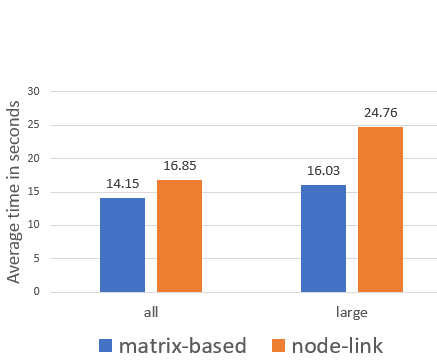
\includegraphics[width=0.35\textwidth]{images/directComparison.PNG}
    \caption{Matrix vs Node-link} 
	\label{directComparison}
\end{wrapfigure}


The research nature of the experiment allowed for thorough data analysis of different factors in the graphs. The results showed that regardless of the graph layout and size the matrix-based graphs (M = 14.15) have better performance than node-link graphs (M = 16.85) for direct questions (Fig\ref{directComparison}) with p-value = 0.0128 (Table\ref{directResults}). When different sizes of each graph type were compared significant difference was found only for the large graphs comparison with matrix-based large graphs (M = 16.03) being easier to read than node-link graphs(M = 24.76). Figure\ref{directComparison} shows the mean values of each each representations. Wilcoxon test showed a p-value of 5.633e-07.



\begin{figure}[!ht]
    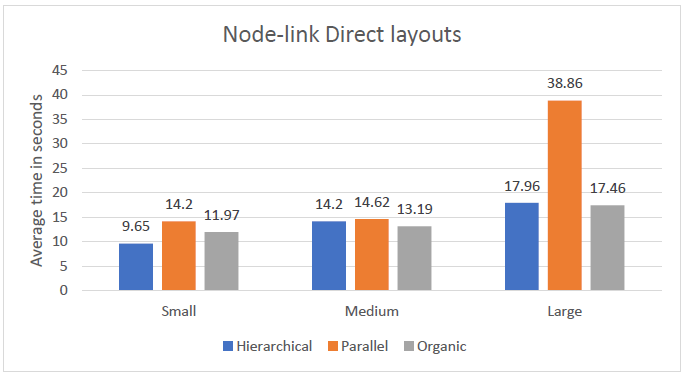
\includegraphics[width=13cm]{images/nodelinkdirectlayouts.PNG}
    \vspace{-15pt}
    \centering
    \caption{Direct Question: Node-link layout comparison in all size groups}
	\label{nodelinkdirectlayouts}
\end{figure}


Node-link layouts were compared in each size group. Figure\ref{nodelinkdirectlayouts} illustrates the difference in mean values in all node-link layouts and sizes. In small size the parallel layout was found the have the worst performance (M = 14.20) and hierarchical layout was found to have the best performance (M = 9.65). Friedman test calculated a p-value of 0.0013* with significant post-hoc tests between all pairs (Table\ref{directResults}). In the medium size measures, the parallel layout had the worst performance time of 15.62 on average, but when Friedman test was conducted no statistical difference between the three layouts was found with p-value = 0.6575. The node-link large size performance time for hierarchical (M=17.96), parallel (M=38.86), and organic (M=17.46) layouts \ref{nodelinkdirectlayouts} was significantly different and has p-value = 3.261e-06*. 

The matrix-based based graphs were not found to have consistent performance differences between the various layouts when direct question was asked. Significant difference was found in the medium size with out degree descending layout (M=12.70) outperforming in degree descending (M=14.64) and alphabetical layouts (M=14.86). As far as the small and the large sizes are concerned p-value was shown to be insignificant.


\begin{table}[H]
\centering
\caption{Direct Question comparisons}
\label{directResults}
\begin{tabular}{|c|c|c|c|c|c|c|}
\hline
\multicolumn{3}{|c|}{\textbf{Matrix}}     & \multicolumn{3}{c|}{\textbf{Node-link}} & \textbf{P-value}              \\ \hline
\multicolumn{3}{|c|}{14.15}               & \multicolumn{3}{c|}{16.85}              & 0.0128*                       \\ \hline
\multicolumn{3}{|c|}{small 10.78}         & \multicolumn{3}{c|}{small 11.92}        & 0.1055                        \\ \hline
\multicolumn{3}{|c|}{medium 14.06}        & \multicolumn{3}{c|}{medium 14.01}       & 0.8776                        \\ \hline
\multicolumn{3}{|c|}{large 16.03}         & \multicolumn{3}{c|}{large 24.76}        & 5.633e-07*                    \\ \hline
\multicolumn{3}{|c|}{\multirow{12}{*}{\cellcolor{gray}}}  & \multicolumn{3}{c|}{small}                                            &\cellcolor{gray} \\ \cline{4-7} 
\multicolumn{3}{|c|}{\cellcolor{gray}}                    & H 9.65      & P 14.20     & O 11.97     & 0.0013*                       \\ \cline{4-7} 
\multicolumn{3}{|c|}{\cellcolor{gray}}                    & H           & P		      &\cellcolor{gray}	& \textless2e-16*               \\ \cline{4-7} 
\multicolumn{3}{|c|}{\cellcolor{gray}}                    & \cellcolor{gray}		& P    		  & O           & 1.8e-09*                      \\ \cline{4-7} 
\multicolumn{3}{|c|}{\cellcolor{gray}}                    & H    	&\cellcolor{gray} & O           & 3.5e-05*                      \\ \cline{4-7} 
\multicolumn{3}{|c|}{\cellcolor{gray}}                    & \multicolumn{3}{c|}{medium}                                            &\cellcolor{gray} \\ \cline{4-7} 
\multicolumn{3}{|c|}{\cellcolor{gray}}                    & H 14.20     & P 14.62     & O 13.19     & 0.6575                        \\ \cline{4-7} 
\multicolumn{3}{|c|}{\cellcolor{gray}}                    & \multicolumn{3}{c|}{large}                                             &\cellcolor{gray} \\ \cline{4-7} 
\multicolumn{3}{|c|}{\cellcolor{gray}}                    & H 17.96     & P 38.86     & O 17.46     & 3.261e-06*                    \\ \cline{4-7} 
\multicolumn{3}{|c|}{\cellcolor{gray}}                    & \cellcolor{gray} & P    & O           & \textless2e-16*               \\ \cline{4-7} 
\multicolumn{3}{|c|}{\cellcolor{gray}}                    & H           & P	&\cellcolor{gray}    & \textless2e-16*               \\ \cline{4-7} 
\multicolumn{3}{|c|}{\cellcolor{gray}}                    & H           & \cellcolor{gray} & O    & 0.001*                        \\ \hline
\multicolumn{3}{|c|}{small}               & \multicolumn{3}{c|}{\multirow{9}{*}{\cellcolor{gray}}}  &                              \cellcolor{gray} \\ \cline{1-3} \cline{7-7} 
inDD 10.35   & outDD 9.25   & alpha 12.75 & \multicolumn{3}{c|}{\cellcolor{gray}}                   & 0.07939                       \\ \cline{1-3} \cline{7-7} 
\multicolumn{3}{|c|}{medium}              & \multicolumn{3}{c|}{\cellcolor{gray}}                   &                              \cellcolor{gray} \\ \cline{1-3} \cline{7-7} 
inDD 14.64   & outDD 12.70  & alpha 14.86 & \multicolumn{3}{c|}{\cellcolor{gray}}                   & \multicolumn{1}{l|}{0.03943*} \\ \cline{1-3} \cline{7-7} 
inDD         & {outDD} &\cellcolor{gray} & \multicolumn{3}{c|}{\cellcolor{gray}}                   & \multicolumn{1}{l|}{2.4e-10*} \\ \cline{1-3} \cline{7-7} 
\cellcolor{gray}& outDD & alpha       & \multicolumn{3}{c|}{\cellcolor{gray}}                   & \multicolumn{1}{l|}{7.5e-07*} \\ \cline{1-3} \cline{7-7} 
inDD &\cellcolor{gray} &  alpha       & \multicolumn{3}{c|}{\cellcolor{gray}}                   & \multicolumn{1}{l|}{0.12}     \\ \cline{1-3} \cline{7-7} 
\multicolumn{3}{|c|}{large}               & \multicolumn{3}{c|}{\cellcolor{gray}}                   & \multicolumn{1}{l|}{\cellcolor{gray}}         \\ \cline{1-3} \cline{7-7} 
inDD 15.34   & outDD 14.76  & alpha 18.00 & \multicolumn{3}{c|}{\cellcolor{gray}}                   & \multicolumn{1}{l|}{0.355}    \\ \hline
\end{tabular}
\end{table}

H - hierarchical P - parallel O - organic inDD - indegree descending outDD - outdegree descending alpha - alphabetical

\subsubsection{Path Questions}


\begin{wrapfigure}{r}{0.35\textwidth}
	\centering
	\vspace{-10mm}
	%\hspace{-8mm}
    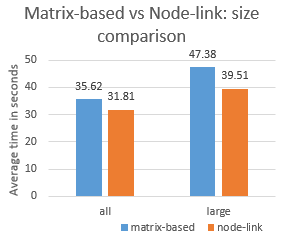
\includegraphics[width=0.35\textwidth]{images/pathComparison.PNG}
    \caption{Matrix vs Node-link} 
	\label{pathComparison}
\end{wrapfigure}

The path question results showed different pattern. The Wilcoxon comparison between the matrix-based (M=35.62) and node-link (M=31.81) representations of any size and layout showed a better performance for node-link graphs \ref{pathComparison} with p-value=0.02479*. In the small group size of this question type, matrix-based representations (M=23.09) were outperformed by node-link graphs (M=27.83). Wilcoxon test reported a p-value of 0.03997* (Table\ref{pathResults}). No difference was found in the medium size graphs, but in the large size group matrix-based graphs (M=47.38) showed worse performance when compared to node-link graphs (M=39.51). Wilcoxon test found a p-value of 0.02847*. 



The node-link layout comparison showed that for small sizes the hierarchical layout (M=27.31) has worst performance, followed by the parallel layout (M=22.43) and the organic layout (M=19.62). Friedman test found a significant difference between the layouts with p-value=5.943e-06*. However, in the medium size group the layouts showed different results (Figure\ref{nodePathLayouts}). The organic layout (M=48.55) performed significantly worse than the parallel (M=26.44) and the hierarchical (M=23.54) \ref{pathResults}. These results were consistent with the large group size layouts where the organic layout (M=47.88) showed worse performance than parallel (M=39.20) and hierarchical (M=31.44) layouts.


\begin{figure}[H]
\centering
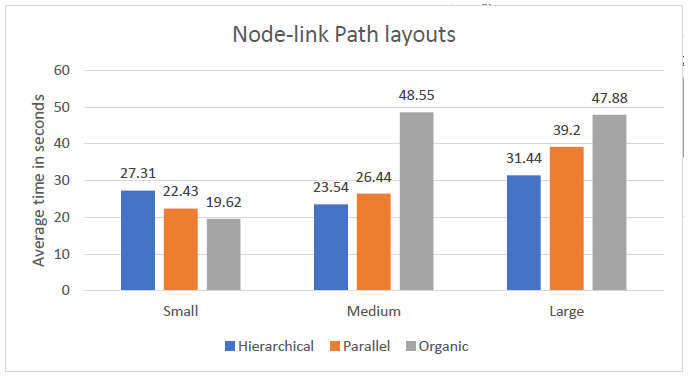
\includegraphics[width=15cm]{images/nodePathLayouts.PNG}
\caption{Path Question: Node-link layout comparison in all size groups}
\label{nodePathLayouts}
\end{figure}

Among the matrix layouts significant difference was found in the small and large size groups. When the size is small, alphabetical layout (M=23.79) outperformed out degree descending (M=29.50) and in degree descending (30.20) layouts \ref{matrixpathlayouts}. A Friedman test found a significant difference between the three layouts with p-value=0.0003245*. In the medium size group, the alphabetical layout was confirmed to have best performance (M=27.29) when compared to in degree descending layout (M=29.07), but not statistical difference was found when compared to out degree descending layout (M=28.68) with p-value= 0.26. No significant difference was found among the layouts in large size. All p-values for path question can be found in Figure \ref{pathResults} 


\begin{figure}[H]
\centering
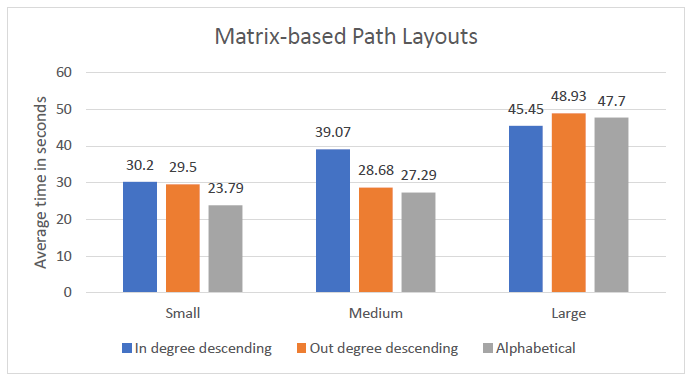
\includegraphics[width=15cm]{images/matrixpathlayouts.PNG}
\caption{Path Question: Matrix-based layout comparison in all size groups}
\label{matrixpathlayouts}
\end{figure}

\begin{table}[H]
\centering
\caption{Path Question comparisons}
\label{pathResults}
\begin{tabular}{|c|c|c|c|c|c|c|}
\hline
\multicolumn{3}{|c|}{\textbf{Matrix}}     & \multicolumn{3}{c|}{\textbf{Node-link}} & \textbf{P-value} \\ \hline
\multicolumn{3}{|c|}{35.62}               & \multicolumn{3}{c|}{31.81}              & 0.02479*         \\ \hline
\multicolumn{3}{|c|}{small 27.83}         & \multicolumn{3}{c|}{small 23.09}        & 0.03997*         \\ \hline
\multicolumn{3}{|c|}{medium 31.67}        & \multicolumn{3}{c|}{medium 32.85}       & 0.2665           \\ \hline
\multicolumn{3}{|c|}{large 47.38}         & \multicolumn{3}{c|}{large 39.51}        & 0.02847*         \\ \hline
\multicolumn{3}{|c|}{\multirow{15}{*}{\cellcolor{gray}}}  & \multicolumn{3}{c|}{small} & \cellcolor{gray}                                 \\ \cline{4-7} 
\multicolumn{3}{|c|}{\cellcolor{gray}}                    & H 27.31      & P 22.43     & O 19.62    & 5.943e-06*       \\ \cline{4-7} 
\multicolumn{3}{|c|}{\cellcolor{gray}}                    & H            & P &\cellcolor{gray}  & 4.5e-12*         \\ \cline{4-7} 
\multicolumn{3}{|c|}{\cellcolor{gray}}                    &\cellcolor{gray} & P     & O          & 4.5e-12 *        \\ \cline{4-7} 
\multicolumn{3}{|c|}{\cellcolor{gray}}                    & H            & \cellcolor{gray} & O   & \textless 2e-16* \\ \cline{4-7} 
\multicolumn{3}{|c|}{\cellcolor{gray}}                    & \multicolumn{3}{c|}{medium}  &\cellcolor{gray}                              \\ \cline{4-7} 
\multicolumn{3}{|c|}{\cellcolor{gray}}                    & H 23.54      & P 26.44     & O 48.55    & 3.08e-09*        \\ \cline{4-7} 
\multicolumn{3}{|c|}{\cellcolor{gray}}                    & H            & P &\cellcolor{gray}   & 2.40e-13*        \\ \cline{4-7} 
\multicolumn{3}{|c|}{\cellcolor{gray}}                    & H & \cellcolor{gray}     & O          & \textless 2e-16* \\ \cline{4-7} 
\multicolumn{3}{|c|}{\cellcolor{gray}}                    & \cellcolor{gray} & P     & O          & \textless 2e-16* \\ \cline{4-7} 
\multicolumn{3}{|c|}{\cellcolor{gray}}                    & \multicolumn{3}{c|}{large} & \cellcolor{gray}                                 \\ \cline{4-7} 
\multicolumn{3}{|c|}{\cellcolor{gray}}                    & H   31.44    & P   39.20   & O  47.88   & 0.0273*          \\ \cline{4-7} 
\multicolumn{3}{|c|}{\cellcolor{gray}}                    & \cellcolor{gray} & P     & O          & 1.1e-09*         \\ \cline{4-7} 
\multicolumn{3}{|c|}{\cellcolor{gray}}                    & H            & P & \cellcolor{gray}   & 1                \\ \cline{4-7} 
\multicolumn{3}{|c|}{\cellcolor{gray}}                    & H & \cellcolor{gray}     & O          & 1.1e-09*         \\ \hline
\multicolumn{3}{|c|}{small}               & \multicolumn{3}{c|}{\multirow{12}{*}{\cellcolor{gray}}} & \cellcolor{gray}                 \\ \cline{1-3} \cline{7-7} 
inDD 30.20   & outDD 29.50  & alpha 23.79 & \multicolumn{3}{c|}{\cellcolor{gray}}                   & 0.0003245*       \\ \cline{1-3} \cline{7-7} 
inDD         & outDD & \cellcolor{gray} & \multicolumn{3}{c|}{\cellcolor{gray}}                   & 1.0e-09*         \\ \cline{1-3} \cline{7-7} 
\cellcolor{gray} & outDD & alpha       & \multicolumn{3}{c|}{\cellcolor{gray}}                   & \textless 2e-16* \\ \cline{1-3} \cline{7-7} 
inDD    &\cellcolor{gray}     & alpha & \multicolumn{3}{c|}{\cellcolor{gray}}                   & 1.7e-07*         \\ \cline{1-3} \cline{7-7} 
\multicolumn{3}{|c|}{medium}              & \multicolumn{3}{c|}{\cellcolor{gray}}                   & \cellcolor{gray}                 \\ \cline{1-3} \cline{7-7} 
inDD 39.07   & outDD 28.68  & alpha 27.29 & \multicolumn{3}{c|}{\cellcolor{gray}}                   & 0.001454*        \\ \cline{1-3} \cline{7-7} 
inDD         & outDD & \cellcolor{gray} & \multicolumn{3}{c|}{\cellcolor{gray}}                   & 4.5e-13*         \\ \cline{1-3} \cline{7-7} 
inDD & \cellcolor{gray} & alpha       & \multicolumn{3}{c|}{\cellcolor{gray}}                   & 7.7e-16*         \\ \cline{1-3} \cline{7-7} 
\cellcolor{gray} & outDD & alpha       & \multicolumn{3}{c|}{\cellcolor{gray}}                   & 0.26             \\ \cline{1-3} \cline{7-7} 
\multicolumn{3}{|c|}{large}               & \multicolumn{3}{c|}{\cellcolor{gray}}                   &\cellcolor{gray}                  \\ \cline{1-3} \cline{7-7} 
inDD 45.45   & outDD 48.93  & alpha 47.7  & \multicolumn{3}{c|}{\cellcolor{gray}}                   & 0.356            \\ \hline
\end{tabular}
\end{table}
H - hierarchical P - parallel O - organic inDD - indegree descending outDD - outdegree descending alpha - alphabetical
\section{Preference Results} 

The participants' answers to the questionnaire brought more light into their graph preference and experience during the experiment. It was found that the majority of people (80\%) would prefer to work with node-link graphs. On the question asking how easy they found working with node-link graphs the participants reported an average of 2 (1="Very easy", 5="Very hard") while for the matrix-based representation an average rating of 2.9 was found. These findings suggest that on average people found working with node-link graphs easier which is consistent with the results for graph preference. On the question whether they enjoy solving logical problems the participants scored an average of 3.8 (1="Not at all" and 5="Very much"). Their liking for Maths on the same scale was averaged to 3.3 meaning that the participants had positive attitude towards problem solving and mathematics. On the last question of whether there was something stopping them from performing at their best most people said "No". However, some participants said that they had issues finding the label they were looking for, some mentioned that they might have experienced difficulties paying attention, while one person just said that they did not find the task particularly interesting. One participant mentioned that the location of the experiment was an issue as there was noise in the environment that was preventing them concentrating properly. Even though the experiment was conducted in the library's quiet area, there were people unaware that different levels of the library require different behaviour, and caused difficulties for this one participant.


\section{Qualitative Results}

The experiment was done in the presence of the researcher to ensure high environmental validity and also to allow for  observations while the participants were doing the tasks. For example, while one of the participants was working on the tasks their telephone rang and they got distracted from the tasks. However, a timer was started to measure how long it took the participant to come back to the tasks and then this time was subtracted from the total recorded time for this question. Additional issue which arises from this event is that it is impossible to measure whether the participant had to read the question again when they came back from their distraction or they were able to continue from where they stopped. Fortunately, this happened only once, and the time before the distraction was added on to the time after the distraction.

In general, there was positive feedback about the questions asked and the nature of the topics. Most people found them very familiar and were interested to find the causal relationships. A small amount of people (N=3) mentioned that the font-size of the labels was small and it was difficult to follow the matrix row and columns on the large graphs because of the small size of the squares. The squares and font-size were made as large as possible, but due to the big amount of information that had to be fitted on one screen, some participants still experienced difficulties. One of these participants said that it might have been more difficult for them as they could have eyesight issues. Other participants were explicitly asked after the experiment whether they had experienced any issues and they reported that everything was fine.

\section{Discussion}

The experimental findings showed that for direct questions matrix graphs have better performance than node-link graphs, but for path questions the opposite was true - node-link graphs outperformed matrix-based representations. Direct questions required the participants to find a label and check which factor is being caused by this label. The results of the experiment suggests that it was easier for the participants to find this label on the matrix-based graph. Considering the layouts of the two representations, the matrix has a row and a column while the node-link layout is rather spread out and unevenly distributed on the screen. Consequently, a possible explanation for the better performance of matrix-based graphs for direct questions can be that it is easier for the human eye to find a label in a row rather than on a flat space where factors are spread out in different directions. 

When path questions were concerned node-link graphs outperformed matrix-based graphs. In order to answer a path question in matrix-based graph two selected cells had to be found which could be positioned on two completely different places in the matrix. Therefore, it would take time for the participant to find these two cells. For node-link graphs, however, the participants were required to follow the link between nodes that are positioned next to each other. Therefore, they had to spend time finding only one of the factors. Our results confirmed the findings of Zekian et al \cite{sheny2007path}, who also concluded that node-link representations are better than matrix-based graphs when answering path questions. 

The layout analysis did not manage to find a consistent best performance layout for all sizes. The node-link layouts in the direct question type consistently reported the parallel layout as the worst performance-wise. 


\chapter{Conclusion}


%%%%%%%%%%%%%%%%
%              %
%  APPENDICES  %
%              %
%%%%%%%%%%%%%%%%
\begin{appendices}

\chapter{Database Schema}

\begin{verbatim}
participants_answers(question_id, participant_id, answer, time)
participants_info(participant_id,participant_name, email, uni_degree, age)
questions(question_id, question, one, two, three, four, correct, image)
\end{verbatim}


\chapter{Running the Programs}
An example of running from the command line is as follows:
\begin{verbatim}
      > java MaxClique BBMC1 brock200_1.clq 14400
\end{verbatim}
This will apply $BBMC$ with $style = 1$ to the first brock200 DIMACS instance allowing 14400 seconds of cpu time.


\chapter{Experimental Stimuli}


\begin{sidewaysfigure}[H]
\centering
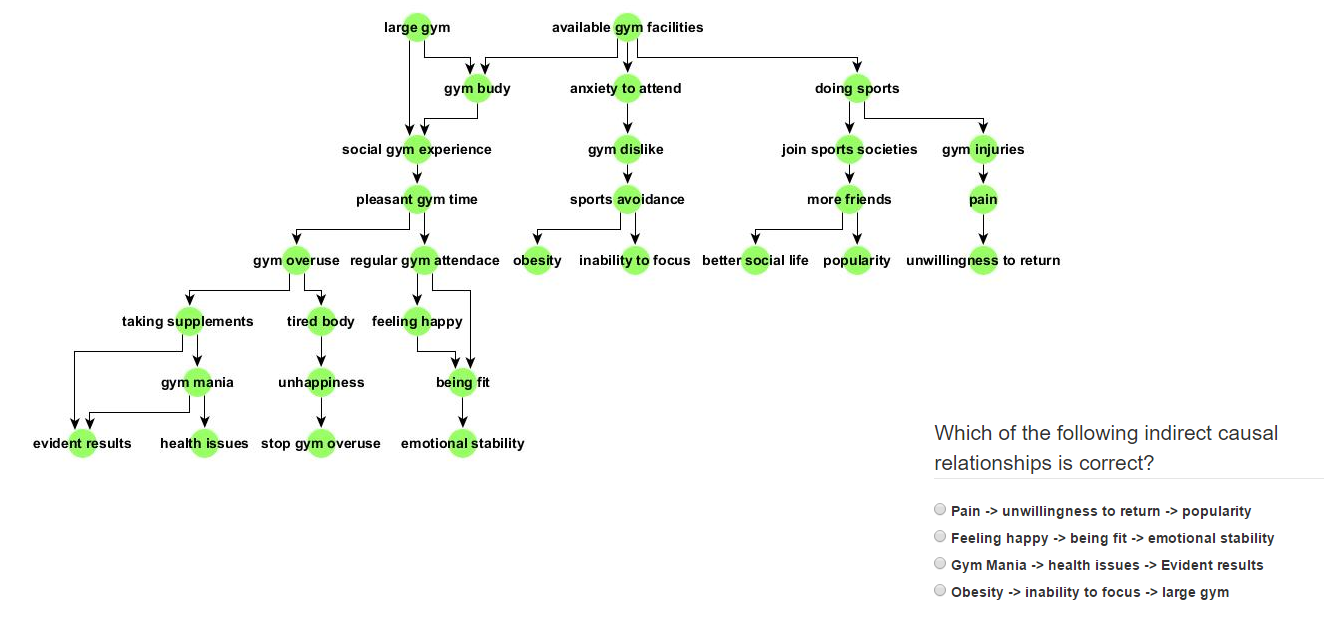
\includegraphics[width=24cm]{exampleQuestion.PNG}
\caption{Example of an experimental question}
\label{exampleQuestion}
\end{sidewaysfigure}


\subsection{Matrix-based}

\begin{figure}[H]
\centering
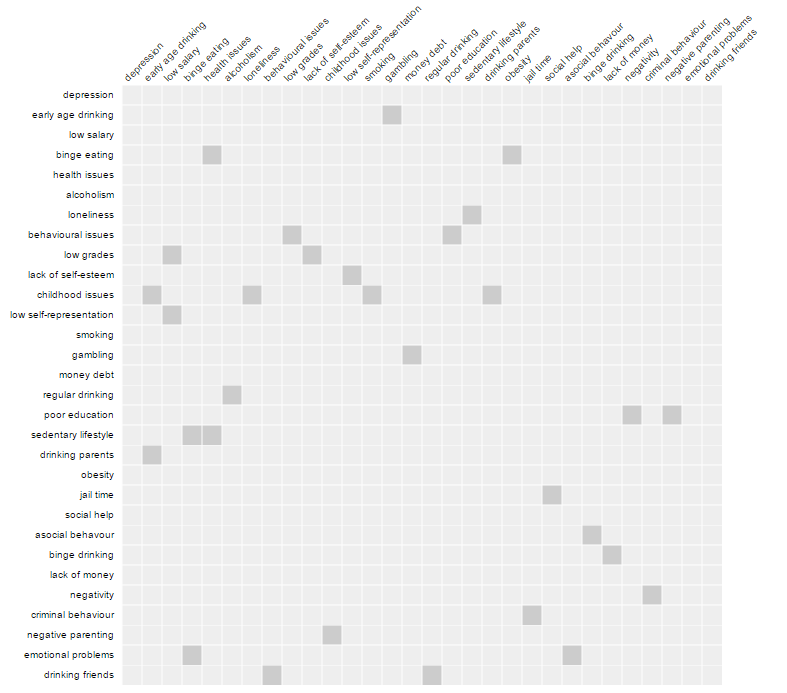
\includegraphics[width=16cm]{images/drinkingLargeInDD.PNG}
\caption{Large matrix-based graph in in degree descending layout and drinking issues domain question}
\label{drinkingLargeInDD}
\end{figure}


\begin{figure}[H]
\centering
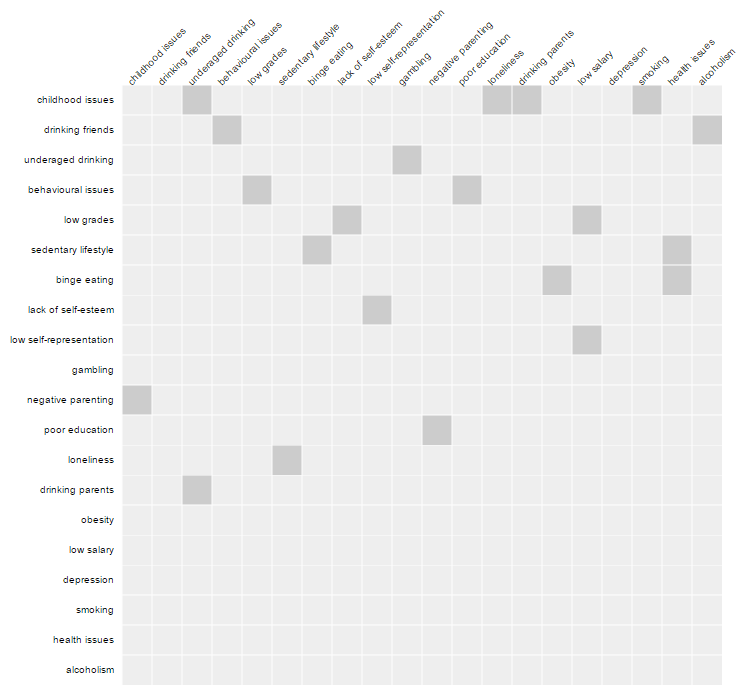
\includegraphics[width=16cm]{images/drinkingMedOutDD.PNG}
\caption{Medium matrix-based graph in out degree descending layout and drinking issues domain question}
\label{drinkingMedOutDD}
\end{figure}

\begin{figure}[H]
\centering
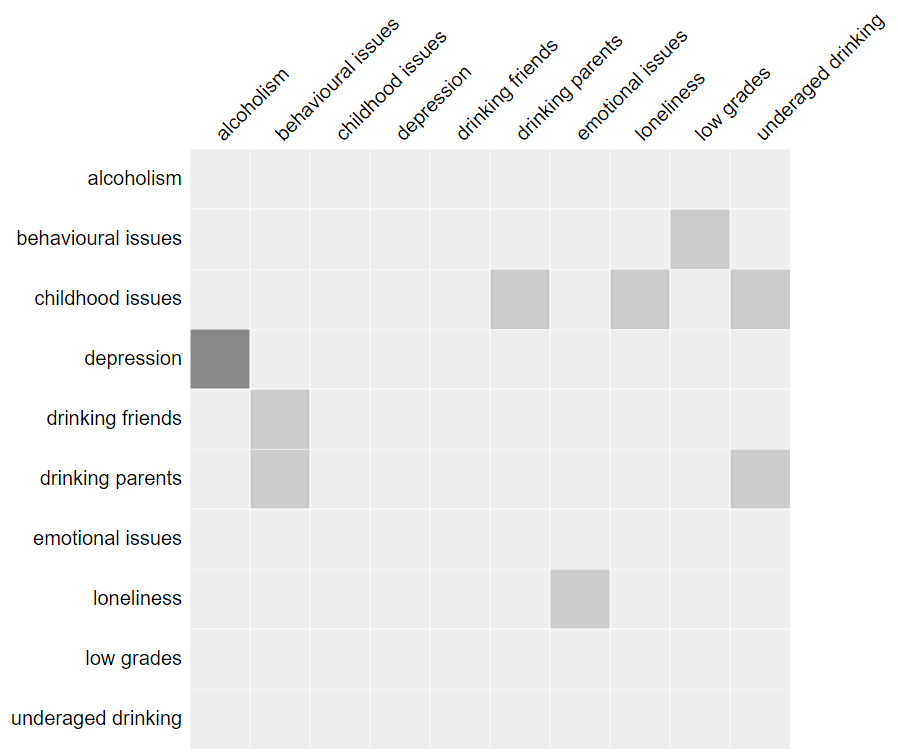
\includegraphics[width=16cm]{images/drinkingSmallAlpha.PNG}
\caption{Small matrix-based graph in alphabetical layout and drinking issues domain question}
\label{drinkingSmallAlpha}
\end{figure}

\begin{figure}[H]
\centering
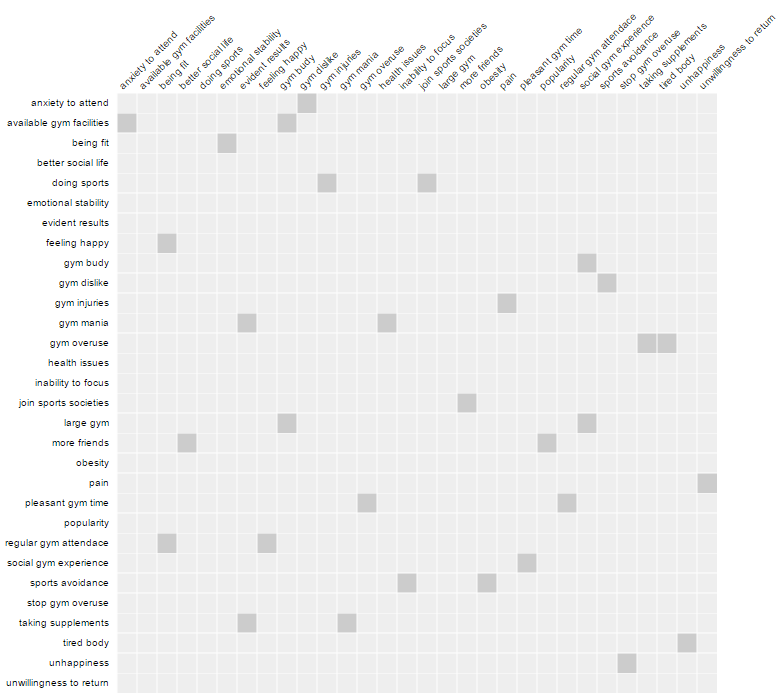
\includegraphics[width=16cm]{images/gymLargeAlpha.PNG}
\caption{Large matrix-based graph in alphabetical layout and sport domain question}
\label{gymLargeAlpha}
\end{figure}


\begin{figure}[H]
\centering
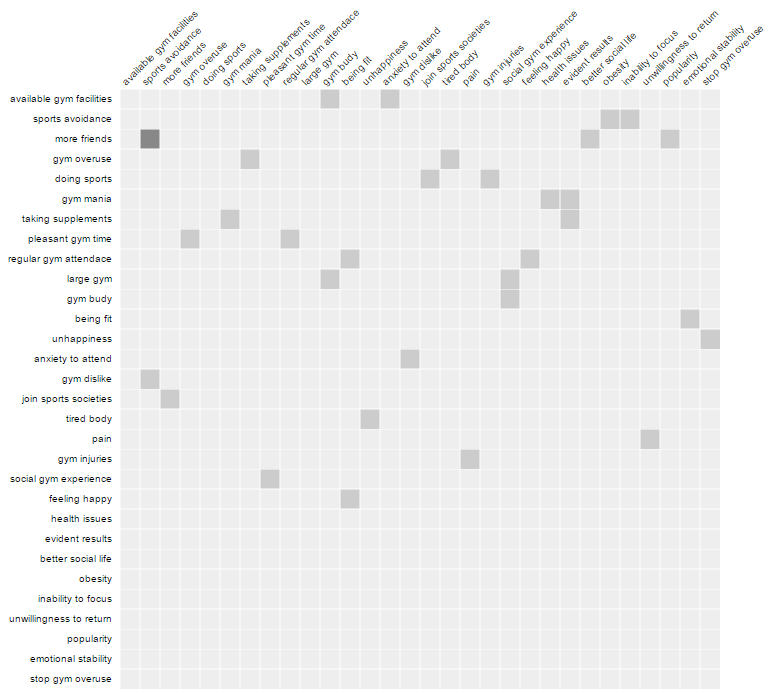
\includegraphics[width=16cm]{images/gymLargeOutDD.PNG}
\caption{Large matrix-based graph in out degree descending layout and drinking issues domain question}
\label{gymLargeOutDD}
\end{figure}

\begin{figure}[H]
\centering
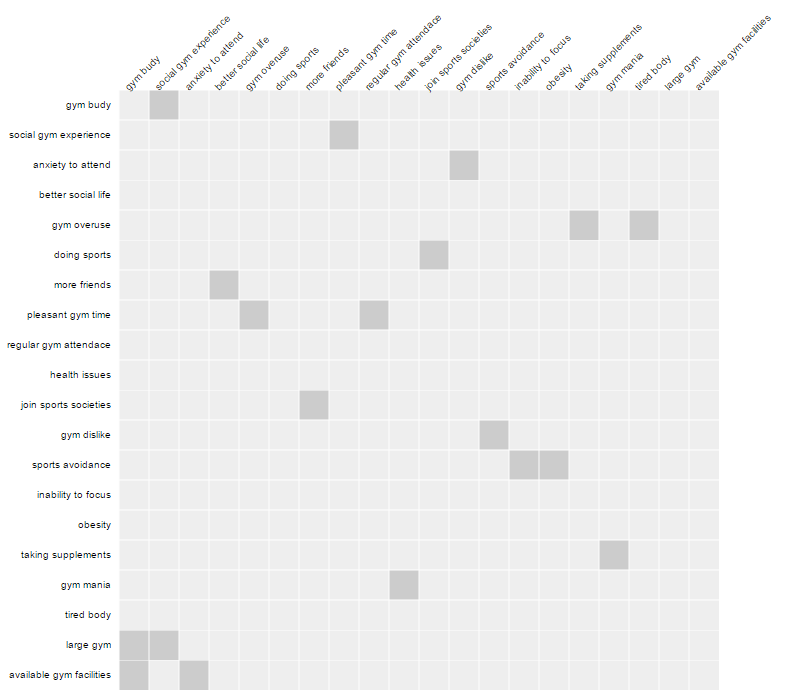
\includegraphics[width=16cm]{images/gymMedInDD.PNG}
\caption{Medium matrix-based graph in in degree descending layout and sport domain question}
\label{gymMedInDD}
\end{figure}

\begin{figure}[H]
\centering
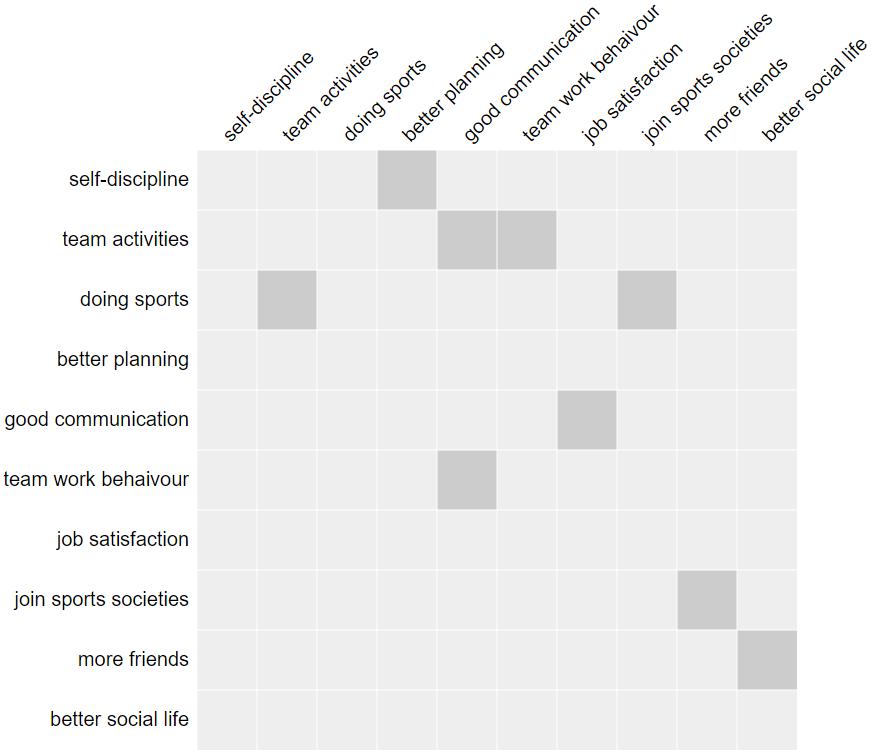
\includegraphics[width=16cm]{images/gymSmallAlpha.PNG}
\caption{Small matrix-based graph in alphabetical layout and sport domain question}
\label{gymSmallAlpha}
\end{figure}


\begin{figure}[H]
\centering
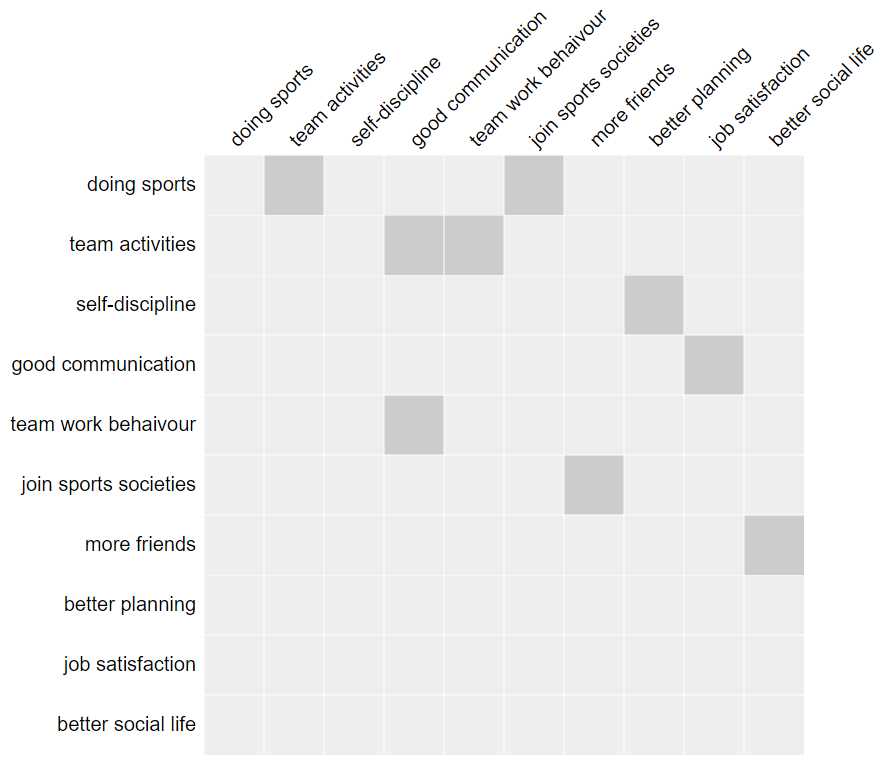
\includegraphics[width=16cm]{images/gymSmallOutDD.PNG}
\caption{Small matrix-based graph in out degree descending layout and sport domain question}
\label{gymSmallOutDD}
\end{figure}



\begin{figure}[H]
\centering
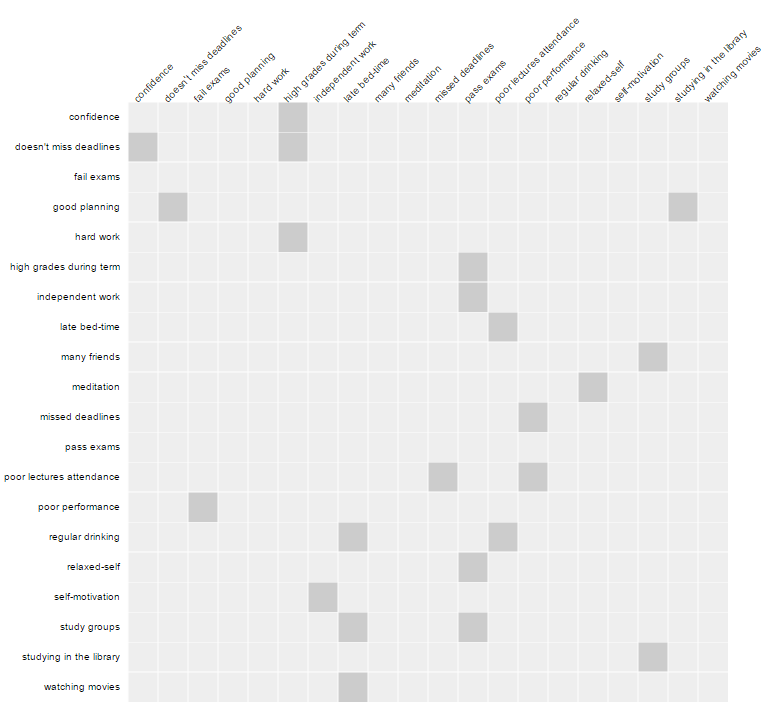
\includegraphics[width=15cm]{images/studentMedAlpha.PNG}
\caption{Medium matrix-based representation in alphabetical layout and student domain question}
\label{studentMedAlpha}
\end{figure}


\begin{figure}[H]
\centering
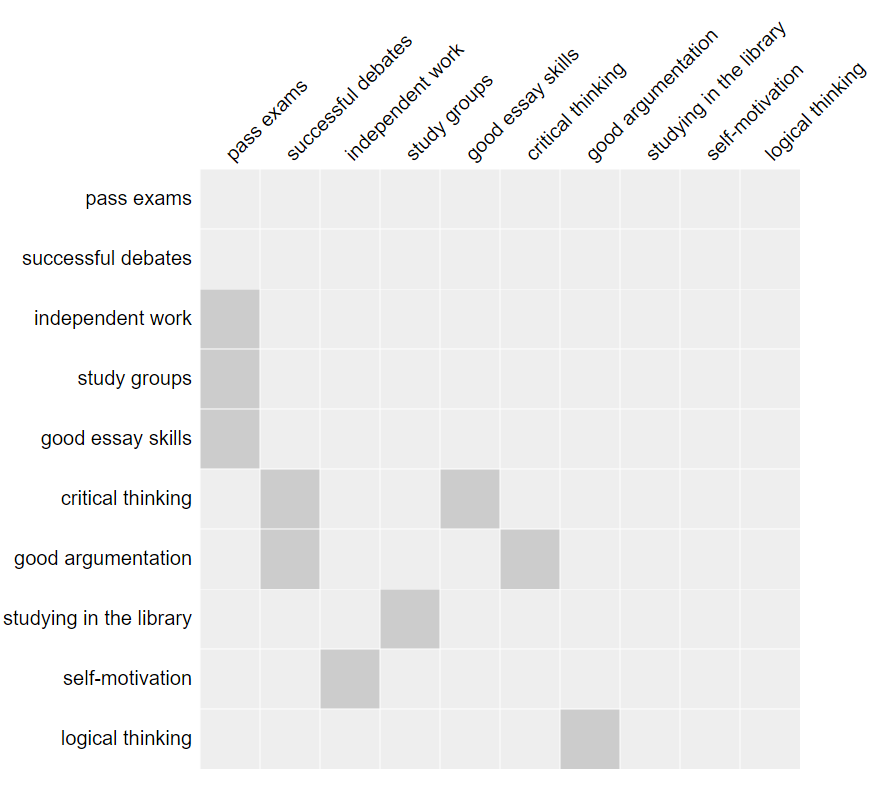
\includegraphics[width=15cm]{images/studentSmallInDD.PNG}
\caption{Small matrix-based representation in in degree descending layout and student domain question}
\label{studentSmallInDD}
\end{figure}

\subsection{Node-link}

\begin{sidewaysfigure}[H]
\centering
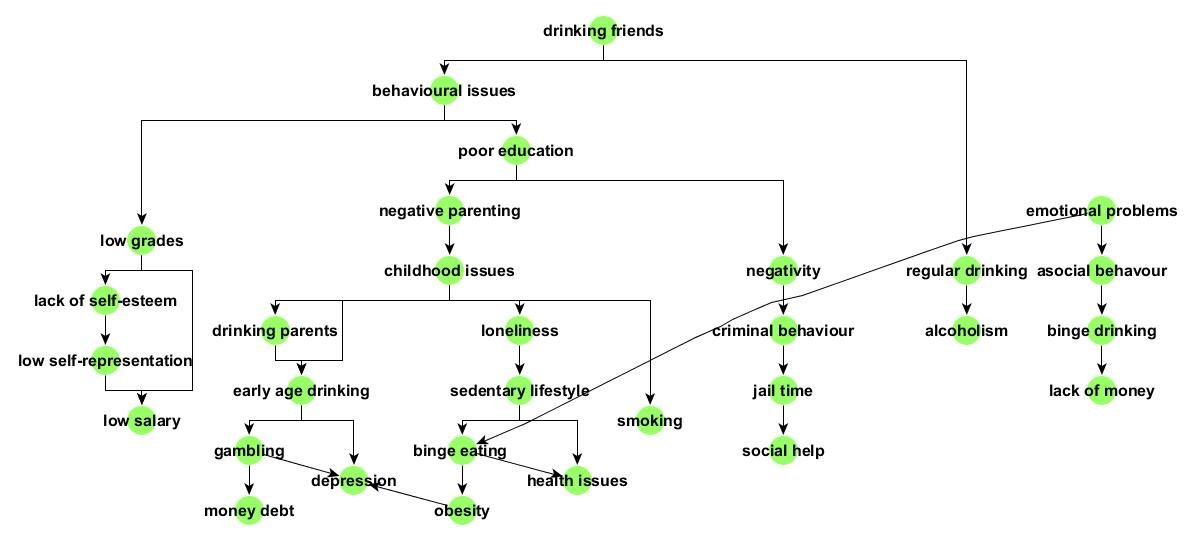
\includegraphics[width=20cm]{images/drinkingIssuesLargeParallel.jpg}
\caption{Large node-link graph in parallel layout and drinking issues domain question}
\label{drinkingIssuesLargeParallel}
\end{sidewaysfigure}

\begin{sidewaysfigure}[H]
\centering
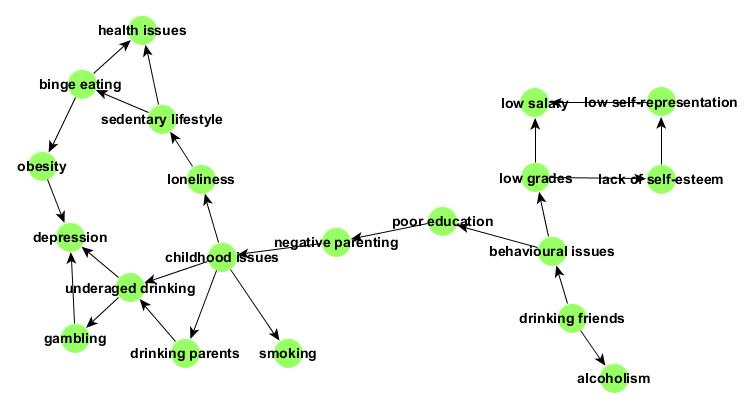
\includegraphics[width=20cm]{images/drinkingIssuesMedOrganic.jpg}
\caption{Medium node-link graph in organic layout and drinking issues domain question}
\label{drinkingIssuesMedOrganic}
\end{sidewaysfigure}


\begin{sidewaysfigure}[H]
\centering
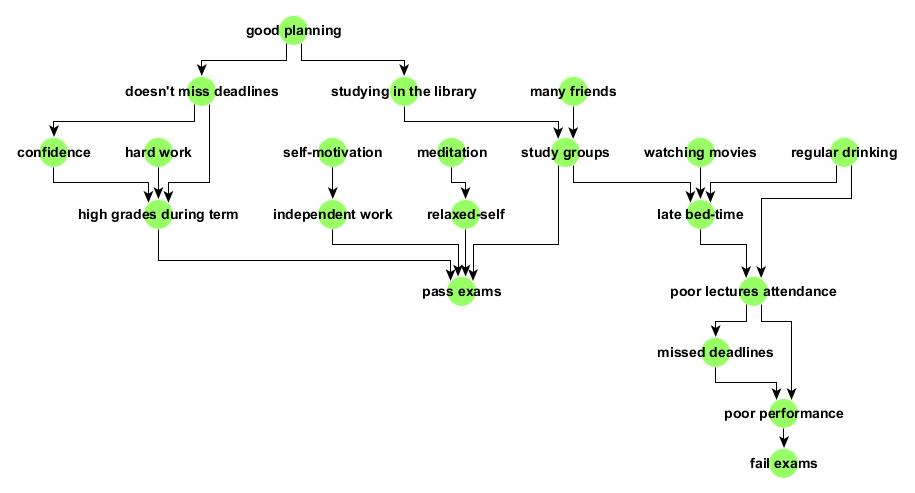
\includegraphics[width=20cm]{images/studentMedHier.jpg}
\caption{Medium matrix-based graph in hierarchical layout and student domain question}
\label{studentMedHier}
\end{sidewaysfigure}


\begin{figure}[H]
\centering
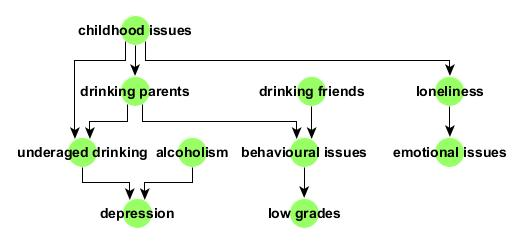
\includegraphics[width=10cm]{images/drinkingIssuesSmallHier.jpg}
\caption{Small node-link graph in hierarchical layout and drinking issues domain question}
\label{drinkingIssuesSmallHier}
\end{figure}


\begin{sidewaysfigure}[H]
\centering
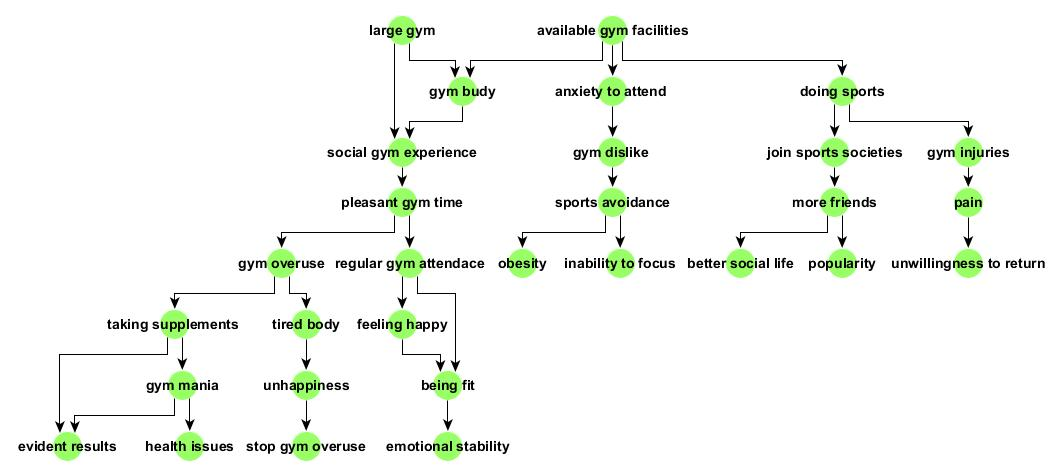
\includegraphics[width=20cm]{images/sportLargeHier.jpg}
\caption{Large node-link graph in hierarchical layout and sport domain question}
\label{drinkingIssuesMedOrganic}
\end{sidewaysfigure}


\begin{sidewaysfigure}[H]
\centering
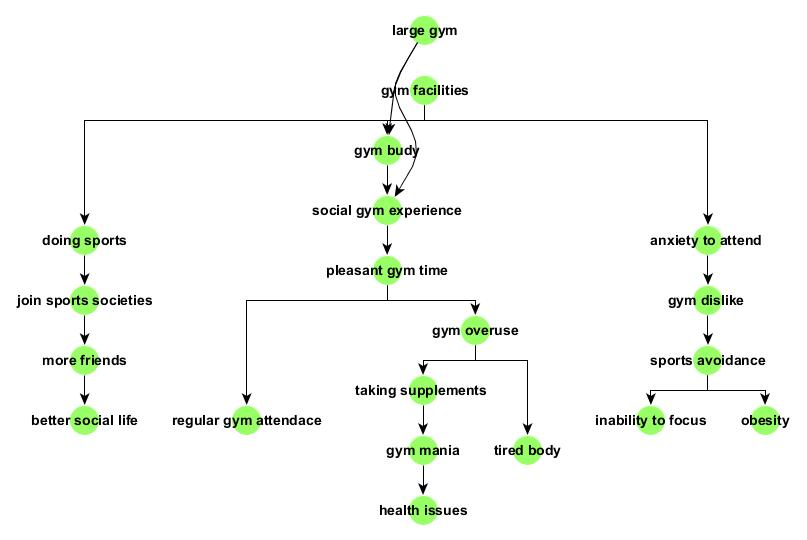
\includegraphics[width=20cm]{images/sportMedParallel.jpg}
\caption{Medium node-link graph in parallel layout and sport domain question}
\label{sportMedParallel}
\end{sidewaysfigure}

\begin{figure}[H]
\centering
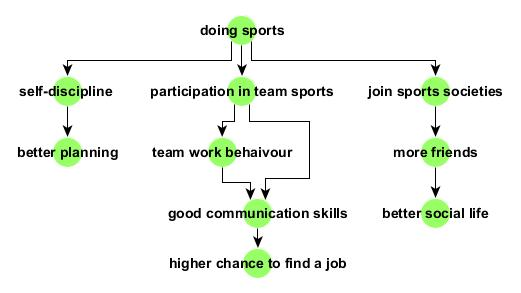
\includegraphics[width=10cm]{images/sportSmallHier.jpg}
\caption{Small node-link graph in hierarchical layout and sport domain question}
\label{sportSmallHier}
\end{figure}


\begin{figure}[H]
\centering
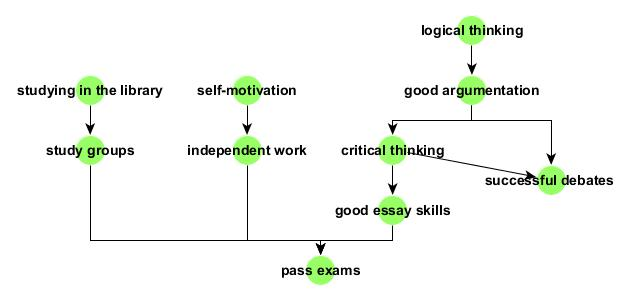
\includegraphics[width=10cm]{images/studentSmallParallel.jpg}
\caption{Small node-link representation in parallel layout and student domain question}
\label{studentSmallInDD}
\end{figure}


\begin{figure}[H]
\centering
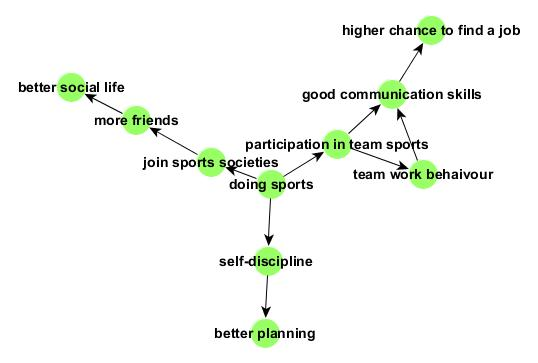
\includegraphics[width=10cm]{images/sportSmallOrganic.jpg}
\caption{Small node-link graph in organic layout and sport domain question}
\label{sportSmallOrganic}
\end{figure}

\begin{figure}[H]
\centering
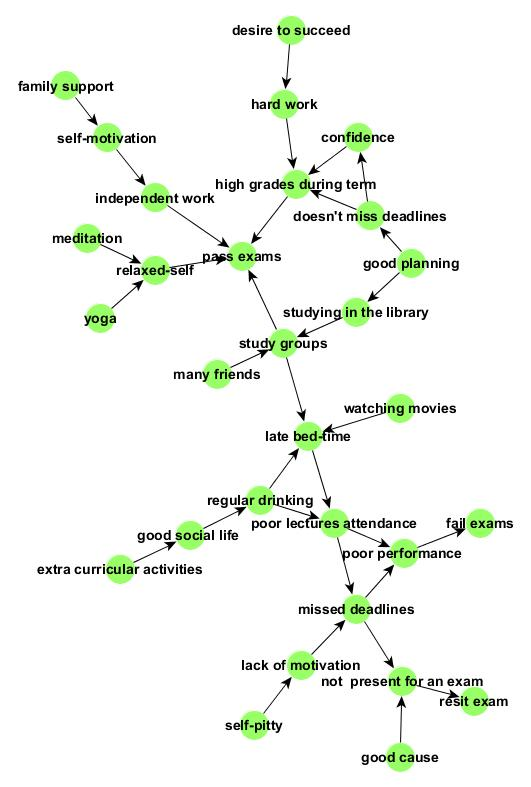
\includegraphics[width=15cm]{images/studentLargeOrganic.jpg}
\caption{Large node-link graph in organic layout and student domain question}
\label{studentLargeOrganic}
\end{figure}



\end{appendices}
%%%%%%%%%%%%%%%%%%%%
%   BIBLIOGRAPHY   %
%%%%%%%%%%%%%%%%%%%%

\bibliographystyle{plain}
\bibliography{bib}

\end{document}
